\chapter{Revision as Biased Choice}\label{ch:4}

Revision operators that satisfy postulate $\ppr{2}$
(besides the more standard postulates $\ppr{1}$ and $\ppr{3-8}$)
can be understood to adopt a particular attitude
towards prior information,
which articulates the policy 
by which the agent's prior information
behaves with respect to new data: 
if new information $\mu$
is consistent with existing beliefs $\phi$, 
then the result of revision is simply $\phi\land\mu$;
in other words, the agent retains its initial beliefs
and simply supplements them with the new item of information,
if it can do so in a consistent way.
Under the choice perspective of belief change 
we have been advocating,
the agent ranks possible outcomes of the revision process
in terms of their plausibility:
in this setting, postulate $\ppr{2}$ 
makes sure that, when beliefs are up for grabs,
models of the prior information $\phi$ are the first in line
to be chosen.
This attitude is in line with a view of revision according to which 
the prior information $\phi$ 
stands for the set of outcomes the agent finds most plausible,
information not to be given up unless challenged
by conflicting new data.
This is a conservative attitude towards initial beliefs,
guided by the desire to preserve them as much as possible.
As pointed out in Section \ref{sec:3-revision},
it is lended support by Peter G\"ardenfors' argument that
information is not cheap and should be preserved to the best
of one's ability \cite[p.\~49]{Gardenfors88}, 
or by Harold Abelson's observation that humans treat beliefs as 
possessions \cite{Abelson86}.
However, it is not the only attitude 
towards the prior information an agent can have.

\begin{figure}\centering
	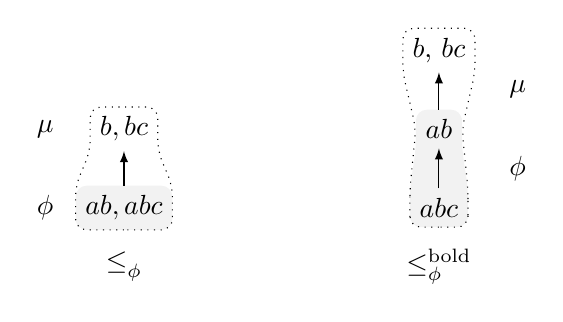
\begin{tikzpicture}
		\node at (0, -0.75){$\le^{\mathrm{\conservative}}_{\phi}$};
		\node at (0,0)(0){$ab,abc$}; 
		\node at (0,1)(1){$b,bc$};
		\node at (-1, 0){$\mods{\phi}$};
		\node at (-1, 1){$\mods{\mu}$};
		\path[-latex] (0) edge (1);
		\fill[opacity = 0.05, rounded corners = 4pt]
			(0.south)--
			(0.south east)--
			(0.east)--
			(0.north east)--
			(0.north)--
			(0.north west)--
			(0.west)--
			(0.south west)--
			(0.south);
		\draw[rounded corners = 4pt, dotted]
			(0.south)--
			(0.south west)--
			(0.west)--
			(0.north west)--
			(1.south west)--
			(1.west)--
			(1.north west)--
			(1.north)--
			(1.north east)--
			(1.east)--
			(1.south east)--
			(0.north east)--
			(0.east)--
			(0.south east)--
			(0.south);

		\node at (4, -0.75){$\le^{\mathrm{bold}}_{\phi}$};
		\node at (4,0)(0){$abc$}; 
		\node at (4,1)(1){$ab$};
		\node at (4,2)(2){$b$, $bc$};
		\node at (5, 0.5){$\mods{\phi}$};
		\node at (5, 1.5){$\mods{\mu}$};
		\path[-latex] (0) edge (1) (1) edge (2);
		\fill[opacity = 0.05, rounded corners = 4pt]
			(0.south)--
			(0.south east)--
			(0.east)--
			(0.north east)--
			(1.south east)--
			(1.east)--
			(1.north east)--
			(1.north)--
			(1.north west)--
			(1.west)--
			(1.south west)--
			(0.north west)--
			(0.west)--
			(0.south west)--
			(0.south);
		\draw[rounded corners = 4pt, dotted]
			(0.south)--
			(0.south west)--
			(0.west)--
			(0.north west)--
			(1.west)--
			(2.south west)--
			(2.west)--
			(2.north west)--
			(2.north)--
			(2.north east)--
			(2.east)--
			(2.south east)--
			(1.east)--
			(0.north east)--
			(0.east)--
			(0.south east)--
			(0.south);
	\end{tikzpicture}
	\caption{
		Two agents start with the same prior information $\phi=a$
		and receive the same new information $\mu=b$,
		but revise according to different preorders:
		$\le^{\conservative}_{\phi}$ is guided by the 
		more conservative imperative of preserving as much
		of the original information as possible;
		$\le^{\bld}_{\phi}$ is bolder, in that it
		considers outcome $abc$ more likely than $ab$, 
		though both are consistent with $\phi$,
		and draws the more specific, though riskier,
		conclusion.
		Models of $\phi$ are shaded in gray,
		models of $\mu$ are surrounded by the dotted line.
	}
	\label{fig:4-asthma-symptoms}
\end{figure}

\begin{xmpl}{The art of diagnosis with biased preferences}{4-asthma-symptoms}
	A patient that has been previously diagnosed with asthma ($a$)
	sees two doctors,
	both of whom are aware of the patient's pre-existing condition.
	After a consultation it emerges that 
	the patient is suffering from shortness of breath ($b$).
	The first doctor revises its beliefs by merely taking in 
	this new information, i.e., concluding
	that the patient suffers from asthma and shortness of breath
	($a\land b$).
	The second doctor infers that chest pain ($c$) 
	must also be present ($a\land b\land c$):
	the two symptoms often go together in asthma, 
	and the doctor is inclined to give added weight 
	to this information.
	The conclusions of both doctors are based on 
	accepting the new information,
	but they follow different strategies: 
	the first doctor is more conservative in the 
	way it uses the new information, 
	whereas the second doctor draws a bolder conclusion.

	Formalizing this as a belief change scenario,
	we would assume
	the alphabet $\Atoms=\{a,b,c\}$
	and two agents, corresponding to the two doctors.
	Both agents are in possession of the same 
	prior information $\phi = a$
	and they both revise
	by the same item of new information $\mu=b$.
	We assume that their revision policies 
	are captured by two $\L$-revision operators 
	$\re^{\conservative}$ and $\re^{\bld}$
	that satisfy postulates $\ppr{1}$ and $\ppr{3-6}$,
	i.e., $\re^{\conservative}$ and $\re^{\bld}$  are exhaustive.
	We know, by Theorem \ref{thm:3-revision-repr-total},
	that this is equivalent to having the doctors
	rank outcomes according to a plausibility order
	specific to each,
	then settle on outcomes
	that are most plausible 
	according to these plausibility orders.
	The first doctor concludes that the patient
	has asthma and shortness of breath,
	i.e., $\phi\re^{\conservative}\mu =a\land b$.
	Note that $\phi\re^{\conservative}\mu\equiv\phi\land\mu$,
	i.e., the first doctor revises in accordance 
	with postulate $\ppr{2}$.
	Since $[\phi\land\mu]=\{ab,abc\}$, this 
	revision policy is equivalent to saying that the
	agent considers outcomes $ab$ and $abc$ equally likely,
	and overall more likely than other models of $\mu$,
	such as $b$ or $bc$.
	Such an attitude is in accordance with an r-faithful 
	$\L$-assignment on interpretations,
	and in particular with properties $\oor{5}$ and $\oor{7}$
	in Section \ref{sec:3-revision}.
	A total preorder $\le^{\conservative}_{\phi}$ consistent with this 
	attitude is depicted on the left in Figure \ref{fig:4-asthma-symptoms}.

	The second doctor concludes that the patient must 
	have chest pain, alongside the 
	already known asthma and shortness of breath,
	i.e., $\phi\re^{\bld}\mu\equiv a\land b\land c$.
	Since $[\phi\land\mu]=\{ab,abc\}$, this 
	revision policy is equivalent to saying that the
	agent considers outcome $abc$ more likely than every other 
	model of $\mu$, including $ab$.
	Such an attitude is not in accordance with an r-faithful 
	$\L$-assignment on interpretations,
	and a total preorder $\le^{\bld}_{\phi}$ consistent with this 
	attitude is depicted on the right in Figure \ref{fig:4-asthma-symptoms}.
	In particular, property $\oor{5}$, saying that models 
	of the prior information $\phi$ should be considered 
	equally likely,
	is not satisfied by $\le^{\bld}_\phi$.
	Nonetheless, in light of its experience, readings
	or hunches, the second doctor is happy to factor in information
	about the relative likelihood of certain outcomes,
	even if it means that they will be at variance with 
	property $\oor{5}$.
\end{xmpl}

Example \ref{ex:4-asthma-symptoms} shows two ways of approaching
revision, based on two ways of ranking outcomes consistent with the
prior information:
a more conservative way, consistent with the familiar postulate $\ppr{2}$,
and a bolder way, more eager to distinguish between such outcomes in terms
of plausibility.
The moral we want to draw from Example \ref{ex:4-asthma-symptoms} 
is not that one of the strategies is 
better, or more rational, than the other, 
since we can, of course, come up with scnearios where 
either of the strategies will fare better than the other.
We also want to resist the conclusion that the right way to model
the difference between these cases is to show that one agent
has access to more information than the other: 
in our setup both agents have access to the same primary information,
$\phi$ and $\mu$; the only thing that differs is the way in which
they rank outcomes consistent with this information.

% One way of thinking
% of postulates $\ppr{1}$ and $\ppr{3-6}$ is that they axiomatize 
% total preorders on interpretations.
% These preorders nominally depend on $\phi$,
% but nothing in postulates $\ppr{1}$ and $\ppr{3-6}$
% touches on how models of $\phi$
% should influence these preorders.
% In other words, there is as yet no information
% about the attitude of an agent towards its initial epistemic state,
% and postulates $\ppr{1}$ and $\ppr{3-6}$ are consistent
% with arbitrary attitudes towards $\phi$.
% including one in which, say, 
% an agent considers models of $\phi$ 
% as the \emph{least} plausible possible worlds.
% Such an attitude towards the models of $\phi$ is, admittedly, 
% extravagant:
% the agent will discard information contained in $\phi$
% at the first possibility to do so. 
% And, while one could be imagine situations in which 
% this behavior makes sense,
% such an attitude challenges the idea that the interpretations
% in $[\phi]$ form the objects of \emph{belief}:
% for, while there is no unanimously agreed upon view about what belief is,
% it can be argued that, at the very least,
% to believe an item of information implies to be partial towards it 
% in certain ways.
% How should the models of $\phi$ stand in relation to
% all other interpretations?
% Example \ref{ex:asthma-symptoms} offers a glimpse into two possible answers:
% the first doctor 
% the agent starts off with some information $\phi$ and differentiates among
% possible worlds consistent with $\phi$: some of these worlds are  more plausible than others,
% perhaps as a result of being more salient, 
% or because of a systematic bias \cite{KahnemanST82}.
% Still, as a whole, models of $\phi$ are more plausible than 
% any \emph{other} interpretations consistent with the new information $\mu$.
% In other words, the agent is biased towards the possible worlds consistent with $\phi$,
% an attitude which fits with the idea of $\phi$ being the agent's \emph{belief}.
% Are there, now, other ways of arranging the models of $\phi$ in $\le_{\phi}$,
% ways that span the space of possible such attitudes?
% We study this question through the lens of additional axioms.

In this chapter we view the attitude
embodied by the standard postulate $\ppr{2}$ 
as one among many that an agent can have 
towards its initial beliefs.
By considering alternatives to
% KM postulate \R{2}, which is 
postulate $\ppr{2}$,
we are able to axiomatize revision operators
that embody a wider range of attitudes towards prior information,
and characterize these operators in terms of the
types of preorders they induce on the set of possible worlds.
To illustrate these principles we provide concrete operators, 
constructed using the ingredients introduced in Section \ref{sec:2-distances}:
a notion of \emph{distance} between interpretations
and an \emph{aggregation function} that ranks possible worlds
depending on the initial beliefs.
We also show, in each case, how these operators fit into the landscape
of new postulates introduced. 
Without the theoretical apparatus of the new postulates,
the concrete operators put forward 
would be merely classified as deviant,
since they do not satisfy 
% KM postulate \R{2}:
the traditional postulate $\ppr{2}$.
But through the present analysis 
they can be viewed as encoding distinct and characterizable 
stances an agent can take towards its beliefs. 

% This chapter is based on work published previously at NMR 2018 \cite{HaretW2018b}
% and IJCAI 2019 \cite{HaretW19a}.

\section{Postulates for biased revision operators}\label{sec:4-postulates}
In Section \ref{sec:3-revision} we presented a set of postulates for revision,
which we divided into several groups.
Postulates $\ppr{1}$ and $\ppr{3-6}$ defined \emph{exhaustive}
revision operators, while postulates $\ppr{1}$, $\ppr{3-5}$ and $\ppr{7-8}$
defined \emph{exclusive} revision operators.
In this chapter we will focus on exhaustive operators,
which, according to Theorem \ref{thm:3-revision-repr-total}, 
are represented by total, syntax insensitive 
$\L$-assignments on interpretations.
The aim here is to hold postulates $\ppr{1}$ and $\ppr{3-6}$ fixed
and explore alternatives to postulate $\ppr{2}$.
We will do this by considering weaker versions of postulate $\ppr{2}$,
as well as postulates that express related, but ultimately different intuitions.

Thus, we put forward the following postulates,
meant to apply to any propositional formulas $\phi$ and $\mu$,
and complete propositional formulas $\dot{\phi}$:

\begin{description}
	\item[($\ppr{9}$)] If $\phi\land\mu$ is consistent, then $\phi\re\mu\models\phi\land\mu$.
	\item[($\ppr{10}$)] If $\phi\land\mu$ is consistent, then $\phi\land\mu\models\phi\re\mu$.
	\item[($\ppr{11}$)] If $\phi\re\mu\models\dual{\phi}$, then $\phi\re\mu\equiv\mu$.
	\item[($\ppr{12}$)] If $\mu\not\models\dual{\phi}$, then $(\phi\re\mu)\land\dual{\phi}$ is inconsistent.
	\item[($\ppr{13}$)] If $\dot{\phi}\models\phi\re\mu$, then $\dot{\phi}\models(\phi\lor\dot{\phi})\re\mu$.
	\item[($\ppr{\NEUT}$)] $\rnm(\phi\re\mu)\equiv\rnm(\phi)\re\rnm(\mu)$.
\end{description}

Each of these postulates encodes a particular type 
of attitude towards prior information,
and they are intended to be thought of in conjunction 
with the basic set of postulates $\ppr{1}$ and $\ppr{3-6}$.
%Notice that, taken together,
%postulates \R{6-7} imply that $\phi\re\mu$ is equivalent to $\phi\land\mu$
%(when $\phi\land\mu$ is consistent).
%This property, alongside postulates \R{1-5}, is 
%typically proposed as the default set of 
%rational properties for revision~\cite{DBLP:journals/ai/KatsunoM92}.
%It should be noted, however, that postulates \R{6-7} 
%embody a particular stance towards initial beliefs $\phi$,
%expounded on below.
%Our purpose in this section is to explore different attitudes 
%an agent can have towards $\phi$,
%and thus we argue for keeping postulates \R{1-5} constant
%and varying the rest.
Postulate $\ppr{9}$ models an agent who reserves the right 
to drop information from $\phi$ if it sees fit to,
even if that information is consistent with $\mu$:
we may imagine this is done on the basis of certain 
preferences over the information encoded by $\phi$,
i.e., the agent is partial towards some of the models 
of $\phi$ to the detriment of others,
along the lines of the second doctor in Example \ref{ex:4-asthma-symptoms}.
This type of discrimination can be explained
by the agent having some background knowledge 
of the relative likelihoods of certain outcomes,
as was the case in Example \ref{ex:4-asthma-symptoms},
or be the result of some heuristic that the agent uses
to process information.

\begin{xmpl}{Steve}{4-heuristic-availability}
	Consider Steve, the subject of a classical example by Daniel Kahneman
	and Amos Tversky:

	\begin{quote}
		An individual has been described by a neighbor as follows: 
		``Steve is very shy and withdrawn, 
		invariably helpful but with little 
		interest in people or in the world of reality. 
		A meek and tidy soul, 
		he has a need for order and structure, 
		and a passion for detail.” 
		Is Steve more likely to be a librarian or a farmer?''
		\cite{Kahneman11}
	\end{quote}
	Most people, we are told, reply that Steve is more likely to be a librarian: 
	they do so based primarily on the stereotypical 
	image of what it is to be a librarian,
	while disregarding more useful facts, such as the statistical distribution of
	librarians versus farmers in the population, which would favor farmers.
	Humans, it seems, readily use a representativeness heuristic to draw 
	conclusions that are otherwise unwarranted.

	Imagine this example simplified to fit the parameters of a quick 
	revision scenario:
	an agent knows that Steve is shy ($a$)
	and learns, in addition, that Steve is helpful and very well organized ($b$).
	The agent concludes that Steve is a librarian ($c$).
	Formally, this example has the same structure as 
	Example \ref{ex:4-asthma-symptoms},
	with prior information $\phi=a$, 
	new information $\mu=b$
	and conclusion $\phi\re\mu\equiv a\land b\land c$,
	and results in the same observation:
	the agent considers the outcome $abc$ more likely than outcome $ab$.
	But this time it is on the basis of an availability bias:
	outcome $abc$ is simply more salient in the agent's mind
	than $ab$ alone, even though they are both consistent with $\phi$ and $\mu$.
	Who are we to judge?
\end{xmpl}

Postulate $\ppr{10}$ refers to an attitude that is, in some ways, 
the oposite of the attitude in postulate $\ppr{9}$: it models an agent who 
incorporates all information in $\phi\land\mu$, 
and possibly extends this to cover more ground.
Taken together, postulates $\ppr{9}$ and $\ppr{10}$ 
imply that $\phi\re\mu$ is equivalent to $\phi\land\mu$, when $\phi\land\mu$ is consistent,
i.e., they are equivalent to the classical postulate $\ppr{2}$.

% This property models an agent 
% who wants to preserve as much of $\phi$ as it can,
% and does not have any bias towards either of the models of $\phi$.
% In the KM postulatestization $\ppr{7}$ and $\ppr{8}$ are packaged together in one postulate
% (i.e., KM postulate $\ppr{2}$) and presented alongside $\ppr{1}$ and $\ppr{3-6}$ as 
% the default set of rational properties for revision \cite{KatsunoM92}.

Postulates $\ppr{11}$ and $\ppr{12}$ focus on the dual formula $\dual{\phi}$
obtained by replacing every literal in $\phi$ with its dual, 
i.e., negated version (see Section \ref{sec:2-prop-logic}).
Why are these formulas significant?
Note that in certain special cases, 
such as when $\phi$ is a conjunction of literals 
or a complete formula (i.e., with exactly one model),
then $\dual{\phi}$ will be a formula whose models are complements of the models of $\phi$.

\begin{xmpl}{Dual formulas as opposite points of view}{4-dual-formula-specific}
	For the set of atoms $\Atoms=\{a,b,c\}$,
	consider formulas 
	$\phi_1 = a\land b\land \lnot c$,
	$\phi_2 = a\land b$,
	$\phi_3 = a\lor b$,
	$\phi_4 = b\rightarrow c$.
	We have that 
	$\dual{\phi_1}=\lnot a\land \lnot b\land c$
	and 
	$\dual{\phi_2} = \lnot a \land \lnot b$,
	with
	$[\phi_1]=\{ab\}$ and $[\phi_2]=\{ab, abc\}$
	while $[\dual{\phi_1}]=\{c\}$ and $[\dual{\phi_2}]=\{\emptyset,c\}$.
	On the other hand, 
	$[\phi_3]=\{a,b,ab,ac,bc,abc\}$ and $[\phi_4]=\{\emptyset,a,c,ac,bc,abc\}$,
	while
	$[\dual{\phi_3}]=\{\emptyset,a,b,c,ac,bc\}$ and $[\dual{\phi_4}] = \{\emptyset,a,b,ab,bc,abc\}$.
	Note that $[\phi_1]\cap[\dual{\phi_1}]=\emptyset$ and $[\phi_2]\cap[\dual{\phi_2}]=\emptyset$,
	but
	$[\phi_3]\cap[\dual{\phi_3}]=\{a,b,ac,bc\}$ 
	and 
	$[\phi_4]\cap[\dual{\phi_4}]=\{\emptyset,a,bc,abc\}$.
\end{xmpl}

Conjunctions of literals or complete formulas can be thought of as being very specific,
in the sense that they model agents with definite opinions on some (or all) atoms.
In this case, $\dual{\phi}$ can be thought of as the point of view opposite to that of $\phi$,
i.e., the outcome least likely to be true if $\phi$ is.
As Example \ref{ex:4-dual-formula-specific} illustrates, however,
this analogy breaks down if $\phi$ is a different type of formula, such as a disjunction or a conditional.
In this case $\phi$ and $\dual{\phi}$ can share models, and the distinction between a formula and its dual
is not as clear-cut anymore.
The claim, then, is only that there are situations in which 
it makes sense to view $\phi$ and $\dual{\phi}$
as embodying opposing stances,
and situations can be imagined in which it is desirable to put bounds on the revision
function in terms of how it treats information encoded by $\dual{\phi}$.
This is the case if the agent has, or is required to have, a definite opinion on every item from an agenda,
as is typically the case in Judgment Aggregation~\cite{Endriss16};
if $\phi$ is a `vivid' formula~\cite{Levesque86};
or, if it encodes something like an agent's preferred bundle from a set of available items.
In all these cases $\phi$ can be required to be a conjunction of literals or a complete formula.
%For our purposes, postulates \ppr9-10} 
%place some bounds on 
%the revision output in terms of the information
%represented by this foreign point of view.
In this context, postulate $\ppr{11}$ says that if $\phi$ undergoes revision by 
a formula $\mu$ embodying such an adverse perspective,
then the agent must adopt $\mu$:
in other words, the agent has no room for maneuvering towards a more amenable middle ground.
% Though this sounds like an odd revision policy,
Such a revision policy makes more sense when considered alongside postulate $\ppr{12}$, %\ppr10},
which specifies that if the agent has the option of believing
states of affairs \emph{not} compatible with $\dual{\phi}$,
it should wholeheartedly adopt those as the most plausible stance.
Taken together, postulates $\ppr{11}$ and $\ppr{12}$
inform the agent to believe states of affairs
compatible with $\dual{\phi}$ only if it has no other choice in the matter:
the models of $\dual{\phi}$
should be part of a viewpoint one is willing to accept
only as a last resort. 

\begin{xmpl}{Recommending as revising}{4-online-recommender}
	Consider an online streaming platform that gathers data about its users
	in order to tailor recommendations to their likes and preferences.
	Suppose $\phi$ encodes something like the information this system 
	has about a specific user (e.g., the items that the user liked), 
	$\mu$ represents a query from the user
	and $\phi\re\mu$ represents the set of results suggested to the user by 
	the online platform, in response to the query $\mu$.

	We can imagine that the platform uses its knowledge $\phi$ to construct 
	a profile of the user, which then serves as guide about what to recommend:
	in revision terms, this profile serves as the revision policy, or, 
	as we will soon see, a ranking of the possible outcomes.
	We can also imagine that it is important for the platform that 
	this profile contains, besides the items that the 
	user is most likely to appreciate, also a list of items that the user will 
	\emph{dislike}, so as to avoid suggesting those as much as possible
	(i.e., unless the user explicitly requests them).
	In revision terms, we can conceptualize this as a set of interpretations that 
	are in the result $\phi\re\mu$ only as a last resort,
	and it is not difficult to see that the duals of the `liked' outcomes 
	are good candidates for these, likely to be loathed, options.
\end{xmpl}

Postulate $\ppr{13}$ enforces coherence of change 
when the prior information includes some element that would have been chosen in a different state of mind,
and is best understood through an example.

\begin{xmpl}{So many options}{4:R13}
	An agent intends to go to an art museum ($a$),
	the beach ($b$) and a concert ($c$),
	encoded as the complete propositional formula $\phi=a\land b\land c$,
	with the set of atoms $\Atoms=\{a,b,c\}$.
	The agent then learns that it only has time
	for one of these activities: this is encoded as newly acquired information
	$\mu = (a\land\lnot b\land \lnot c)\lor (\lnot a\land b\land \lnot c)\lor (\lnot a\land\lnot b\land c)$,
	with $[\mu]=\{a,b,c\}$.
	The agent chooses the art museum $a$, i.e.,
	$\phi\re\mu\equiv\dot{\phi}\equiv a\land\lnot b\land\lnot c$.
	Note that $\dot{\phi}\models\phi\re\mu$.
	If the agent's initial intentions had been more inclusive
	in the sense that it would have expressed a willingness to do either all three activities
	or just visit the museum, 
	encoded as $\phi\lor\dot{\phi}$,
	then, faced with the same new information $\mu$, 
	the option of going to the art museum
	(i.e., $a\land\lnot b\land\lnot c$) should still feature as one of its most preferred options.
\end{xmpl}

We have also found it suitable to add here a neutrality postulate $\ppr{\NEUT}$, 
requiring that a revision operator does not favor propositional atoms based solely on their names.
This idea is expressed by requiring the revision output to be invariant under a renaming $\rnm$ of atoms,
and, in conjunction with the insensitivity to syntax postulate $\ppr{4}$,
it is perhaps natural to expect it from any revision operator.
The inspiration for postulate $\ppr{\NEUT}$ is
the social choice literature
and, though it has appeared in belief change before, 
under various guises~\cite{HerzigR99,MarquisS14,HaretPW16}, 
neutrality usually goes unstated in standard presentations of revision.

\section{Biased preferences over outcomes}\label{sec:4-assignments}
A clearer view of postulates $\ppr{9-13}$ and $\ppr{\NEUT}$
emerges when looking at the constraints they impose on how models of $\phi$
are placed in the preorder $\le_\phi$.
That is to say, we assume an agent with prior information $\phi$ ranks interpretations
in a total preorder $\le_\phi$,
i.e., that there exists a total, syntax insensitive $\L$-assignment 
$\as$ on interpretations
that satisfies properties $\oor{1-4}$, as presented in Section \ref{sec:3-revision}.
The additional constraints we want to consider in this chapter
are expressed in the following properties,
applying for any interpretations $w_1$, $w_2$ and $v$
and propositional formulas $\phi$ and $\px_v$, where $[\px_v]=\{v\}$:

\begin{description}
	\item[($\oor{7}$)] If $w_1\in[\phi]$ and $w_2\notin[\phi]$, then $w_1<_\phi w_2$.

	\item[($\oor{8}$)] If $w_1\in[\phi]$, then $w_1\le_\phi w_2$.
		
	\item[($\oor{9}$)] If $w_1\in[\dual{\phi}]$, then $w_2\le_\phi w_1$.
	
	\item[($\oor{10}$)] If $w_1\in[\dual{\phi}]$ and $w_2\notin[\dual{\phi}]$, then $w_2<_\phi w_1$.
	
	\item[($\oor{11}$)] If $v\le_\phi w$, then $v\le_{\phi\lor\px_v} w$.
	
	\item[($\oor{\NEUT}$)] If $w_1\le_\phi w_2$, then $\rnm(w_1)\le_{\rnm(\phi)}\rnm(w_2)$.	
\end{description}

% A revision operator is \emph{basic} if it satisfies postulates 
% $\ppr{1,3-5}$ and \emph{neutral} if it satisfies postulate $\ppr\NEUT$.
\begin{figure}\centering
	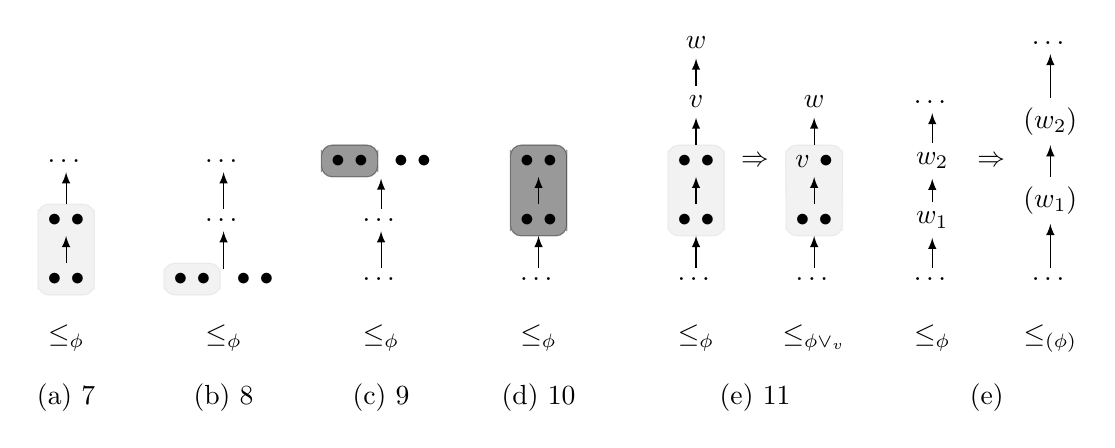
\begin{tikzpicture}
		\node at (0,-1.5){(a) $\oor{7}$}; 
		\node at (0,-0.75){$\le_\phi$};
		\node at (0,0)(0){$\bullet~\bullet$};
		\node at (0,0.75)(1){$\bullet~\bullet$};
		\node at (0,1.5)(2){\dots};
		\path[-latex] (0) edge (1)(1) edge (2);
		\fill[draw, opacity=0.05, rounded corners=4pt]
		(0.south)--
		(0.south west)--
		(0.west)--
		(1.west)--
		(1.north west)--
		(1.north)--
		(1.north east)--
		(1.east)--
		(0.east)--
		(0.south east)--
		(0.south);

		\node at (2,-1.5){(b) $\oor{8}$}; 
		\node at (2,-0.75){$\le_\phi$};
		\node at (1.6,0)(0){$\bullet~\bullet$};
		\node at (2.4,0)(1){$\bullet~\bullet$};
		\node at (2,0)(a1){};
		\node at (2,0.75)(2){\dots};
		\node at (2,1.5)(3){\dots};
		\path[-latex] (a1) edge (2)(2) edge (3);
		\fill[draw, opacity=0.05, rounded corners=4pt]
		(0.north)--
		(0.north east)--
		(0.east)--
		(0.south east)--
		(0.south)--
		(0.south west)--
		(0.west)--
		(0.north west)--
		(0.north);

		\node at (4,-1.5){(c) $\oor{9}$}; 		
		\node at (4,-0.75){$\le_\phi$};
		\node at (3.6,1.5)(0){$\bullet~\bullet$};
		\node at (4.4,1.5)(1){$\bullet~\bullet$};
		\node at (4,1.4)(a1){};
		\node at (4,0.75)(2){\dots};
		\node at (4,0)(3){\dots};
		\path[-latex] (2) edge (a1)(3) edge (2);
		\fill[draw, opacity=0.4, rounded corners=4pt]
		(0.north)--
		(0.north east)--
		(0.east)--
		(0.south east)--
		(0.south)--
		(0.south west)--
		(0.west)--
		(0.north west)--
		(0.north);

		\node at (6,-1.5){(d) $\oor{10}$}; 		
		\node at (6,-0.75){$\le_\phi$};
		\node at (6,1.5)(0){$\bullet~\bullet$};
		\node at (6,0.75)(1){$\bullet~\bullet$};
		\node at (6,0)(2){\dots};
		\path[-latex] (2) edge (1)(1) edge (0);
		\fill[draw, opacity=0.4, rounded corners=4pt]
		(0.north)--
		(0.north west)--
		(0.west)--
		(1.west)--
		(1.south west)--
		(1.south)--
		(1.south east)--
		(1.east)--
		(0.east)--
		(0.north east)--
		(0.north);

		\node at (8.75,-1.5){(e) $\oor{11}$}; 		
		\node at (8,-0.75){$\le_\phi$};
		\node at (8,0)(d){\dots};
		\node at (8,0.75)(k1){$\bullet~\bullet$};
		\node at (8,1.5)(k2){$\bullet~\bullet$};
		\node at (8,2.25)(wp){$v$};
		\node at (8,3)(w){$w$};
		
		\node at (8.75, 1.5){$\Rightarrow$};
		
		\node at (9.5,-0.75){$\le_{\phi\lor\px_v}$};		
		\node at (9.5,0)(d1){\dots};
		\node at (9.5,0.75)(wp1){$\bullet~\bullet$};
		\node at (9.5,1.5)(wp2){$v~\bullet$};
		\node at (9.5,2.25)(w1){$w$};
		
		\path[-latex] 
		(d)edge(k1)(k1)edge(k2)(k2)edge(wp)(wp) edge (w)
		(d1)edge(wp1)(wp1)edge(wp2)(wp2)edge(w1);
		\fill[draw, opacity=0.05, rounded corners=4pt]
		(k1.south)--(k1.south west)--(k1.west)--(k2.west)--
		(k2.north west)--(k2.north)--(k2.north east)--
		(k2.east)--(k1.east)--(k1.south east)--(k1.south);
		\fill[draw, opacity=0.05, rounded corners=4pt]
		(wp1.south)--(wp1.south west)--(wp1.west)--(wp2.west)--
		(wp2.north west)--(wp2.north)--(wp2.north east)--
		(wp2.east)--(wp1.east)--(wp1.south east)--(wp1.south);

		\node at (11.75,-1.5){(e) $\oor{\NEUT}$}; 		
		\node at (11,-0.75){$\le_\phi$};
		\node at (11,0)(d){\dots};
		\node at (11,0.75)(1){$w_1$};
		\node at (11,1.5)(2){$w_2$};
		\node at (11,2.25)(3){\dots};
		
		\path[-latex]
			(d)edge(1)(1)edge(2)(2)edge(3);

		\node at (11.75, 1.5){$\Rightarrow$};
		
		\node at (12.5,-0.75){$\le_{\rnm(\phi)}$};		
		\node at (12.5,0)(d){\dots};
		\node at (12.5,1)(1){$\rnm(w_1)$};
		\node at (12.5,2)(2){$\rnm(w_2)$};
		\node at (12.5,3)(3){\dots};

		\path[-latex]
			(d)edge(1)(1)edge(2)(2)edge(3);
	\end{tikzpicture}
	\caption{
		Schematic view of prototypical preorders
		satisfying each of the properties $\oor{6-10}$;
		models of $\phi$ are in the light gray area,
		models of $\dual{\phi}$ are in the dark gray area.}
	\label{fig:4-biased-preorders-schematic}	
\end{figure}

Each of properties $\oor{7-11}$ tells us something about how prior information $\phi$ 
biases a plausibility ordering over outcomes, especially with regards to the outcomes consistent with $\phi$ 
(i.e., models of $\phi$),
whereas the neutrality property $\oor{\NEUT}$ 
tells us something about the kind of bias the ordering should avoid.
A schematic view of these preorders is offered in 
Figure \ref{fig:4-biased-preorders-schematic}.
Property $\oor{7}$, depicted in Figure~\ref{fig:4-biased-preorders-schematic}-(a), 
says that models of $\phi$ are generally considered
more plausible than interpretations that do not satisfy $\phi$,
but models of $\phi$ themselves may not be equally plausible relative to each other.
Property $\oor{7}$ is familiar from Section \ref{sec:3-revision}, though 
there it was always considered in conjunction with
$\oor{5}$ or $\oor{6}$, and never by itself. Here we shine a spotligh on it alone.
Property $\oor{8}$, depicted in Figure~\ref{fig:4-biased-preorders-schematic}-(b), says that
models of $\phi$ are minimal elements in $\phi$, 
though possibly not uniquely so.
Note that property $\oor{8}$ implies property $\oor{6}$ (see Section \ref{sec:3-revision}),
which says that models of $\phi$ should be equally plausible in $\le_\phi$:
however, $\oor{8}$ tells us more than $\oor{5}$:
it tells us that the agent not only considers models of $\phi$ as equally plausible,
but also at least as plausible as any other outcome.
Properties $\oor{9-10}$, depicted in Figure~\ref{fig:4-biased-preorders-schematic}-(c,d),
say that models of the dual formula $\phi$ are the least plausible interpretations in $\le_\phi$,
while property $\oor{11}$, depicted in Figure~\ref{fig:4-biased-preorders-schematic}-(e),
says that if $v$ is more plausible than $w$ when
the initial beliefs are $\phi$, then $v$ would still be more plausible 
than $w$ if it were part of the initial beliefs.
Lastly, the neutrality property $\oor{\NEUT}$ says that the ranking $\le_\phi$ should be invariant
when renaming the atoms.

Note that properties $\oor{7-8}$, together,
are equivalent to property $\oor{6}$, presented in Section \ref{sec:3-revision}.
Thus, properties $\oor{7-8}$
together with the standard properties 
$\oor{1-5}$ define what is more commonly known as 
a \emph{faithful assignment} \cite{KatsunoM92},
or, as we have named it here,
a total, syntax independent r-faithful $\L$-assignment on interpretations.
Such an assignment
places all and only models of $\phi$ on the lowest level of $\le_\phi$,
and corresponds to an agent for which outcomes 
consistent with its prior belief are the most plausible states of affairs.
This attitude, as is apparent here, 
arises out of a combination of two attitudes that can be looked at separately.

Properties $\oor{7-11}$ and $\oor{\NEUT}$ 
turn out to characterize postulates $\ppr{9-13}$ and $\ppr{\NEUT}$ 
on the semantic level,
as per the following representation result.
Recall that an $\L$-revision operator $\re$ is
represented by an $\L$-assignment $\as$ on interpretations
if $[\phi\re \mu] = \min_{\le_\phi}[\mu]$, for any propositional formulas $\phi$ and $\mu$,
and that, by Theorem \ref{thm:3-revision-repr-total},
if $\re$ is exhaustive, then there always exists a total
assignment $\as$ (i.e., such that $\le_\phi$ is a total preorder) representing it.
Recall, as well, that the $\L$-proxy of a pair $\{w_1,w_2\}$ of interpretations is
a propositional formula $\px_{1,2}$ 
for which $[\px_{1,2}]=\{w_1,w_2\}$.

\begin{thm}{}{4-biased-revision-repr}
	If $\re$ is revision operator that 
	satisfies postulates $\ppr{1}$ and $\ppr{3-6}$
	(i.e., is exhaustive)
	and $\as$ is a total, syntax insensitive 
	$\L$-assignment on interpretations
	that represents it,
	then the following equivalences hold:
	\begin{description}
		\item[(1)] $\re$ satisfies postulate $\ppr{9}$ iff $\as$ satisfies property $\oor{7}$;
		\item[(2)] $\re$ satisfies postulate $\ppr{10}$ iff $\as$ satisfies property $\oor{8}$;
		\item[(3)] $\re$ satisfies postulate $\ppr{11}$ iff $\as$ satisfies property $\oor{9}$;
		\item[(4)] $\re$ satisfies postulate $\ppr{12}$ iff $\as$ satisfies property $\oor{10}$;
		\item[(5)] $\re$ satisfies postulate $\ppr{13}$ iff $\as$ satisfies property $\oor{11}$;
		\item[(6)] $\re$ satisfies postulate $\ppr{\NEUT}$ iff $\as$ satisfies property $\oor{\NEUT}$.
	\end{description}
\end{thm}

\begin{prf*}{}{}%
	We start with Equivalence 1 and show each direction in turn.

	(``$\Leftarrow$'')
	Take a total $\L$-assignment $\as$ on interpretations 
	satisfying property $\oor{7}$
	and the revision operator $\re$ represented by it.
	We want to show that $\re$ satisfies postulate $\ppr{9}$,
	and start by assuming that $\phi\land\mu$ is consistent.
	This implies that $\mu$ is consistent and, by postulate $\ppr{3}$,
	that $\phi \re \mu$ is consistent as well.
	Take, then, an interpretation $w$ such that $w\in[\phi\re\mu]$,
	and suppose $w\notin[\phi\land\mu]$.
	Since $[\phi\re\mu]=\min_{\le_\phi}[\mu]$,
	we obtain that $w\in\min_{\le_\phi}[\mu]$
	and hence $w\in[\mu]$.
	Thus, the fact that $w\notin[\phi\land\mu]$
	implies that $w\notin[\phi]$.
	But, by assumption, it holds that $[\phi\land\mu]\neq\emptyset$,
	which means that there exists $w'\in[\phi\land\mu]$
	and, by property $\oor{7}$, it follows that $w'<_\phi w$.
	But we also have that $w\in\min_{\le_\phi}[\mu]$:
	since $\le_\phi$ is total, this implies that $w \le_\phi w'$: we have arrived at a contradiction.
	
	(``$\Rightarrow$'')
	Take an exhaustive revision operator $\re$ additionally satisfying postulate $\ppr{9}$
	and a total $\L$-assignment $\as$ on interpretations that represents it.
	To show that $\le_\phi$ satisfies property $\oor{7}$, 
	take interpretations $w_1$ and $w_2$ such that $w_1\in[\phi]$
	and $w_2\notin[\phi]$.
	We then have that $\phi\land\px_{1,2}$ is consistent
	and hence, by postulate $\ppr{9}$,
	that $\phi\re\px_{1,2}\models\phi\land\px_{1,2}$.
	Since $[\phi\re\px_{1,2}]$ is, by postulates $\ppr{1}$ and $\ppr{3}$,
	a non-empty subset of $[\px_{1,2}]=\{w_1,w_2\}$,
	we have that at least one of $w_1$ and $w_2$ is in $[\phi\re\px_{1,2}]$.
	Notice, now, that we cannot have $w_2\in[\phi\re\px_{1,2}]$,
	since it would follow that $w_2\in\mods{\phi\land\px_{1,2}}$ and,
	\emph{a fortiori}, that $w_2\in[\phi]$,
	which contradicts a previous finding.
	Thus, $[\phi\re\px_{1,2}]=\set{w_1}$.
	Since $\le_\phi$ represents $\re$, 
	we have that
	$[\phi\re\px_{1,2}]=\min_{\le_\phi}[\px_{1,2}]=\{w_1\}$,
	i.e., that $w_1<_\phi w_2$.		
	
	For Equivalence 2, we show again each direction in turn.

	(``$\Leftarrow$'')
	Take, first, a total $\L$-assignment $\as$ on interpretations 
	satisfying property $\oor{8}$,
	and the revision operator $\re$ represented by it.
	% We want to show that $\re$ satisfies postulate $\ppr{10}$.
	Assuming that $\phi\land\mu$ is consistent,
	we want to show that for any $w_1\in[\phi\land\mu]$, it holds that $w_1\in[\phi\re\mu]$ as well.
	Since $\re$ is represented by $\as$, this is equivalent to showing that
	$w\in\min_{\le_\phi}[\mu]$.
	Take, then, an interpretation $w\in[\phi\land\mu]$,
	and an arbitrary interpretation $w'\in[\mu]$.
	Applying property $\oor{8}$, we infer that $w_1 \le_\phi w_2$,
	which then implies that $w\in\min_{\le_\phi}[\mu]$.

	(``$\Rightarrow$'')
	Take an exhaustive revision operator $\re$ that additionally satisfies postulate $\ppr{10}$,
	and a total $\L$-assignment $\as$ on interpretations that represents it.
	To show that $\le_\phi$ satisfies property $\oor{8}$,
	take two interpretations $w_1$ and $w_2$
	such that $w_1\in[\phi]$. 
	Then, by postulate $\ppr{10}$, we have that 
	$\phi\land\px_{1,2}\models\phi\re\px_{1,2}$.
	This implies that $w_1\in[\phi \re \px_{1,2}]$,
	i.e., that $w_1\in\min_{\le_\phi}[\px_{1,2}]$.
	Thus, it holds that $w_1\le_\phi w_2$.

	Equivalences 3 and 4 are analogous to 1 and 2, respectively.
	For Equivalence 5, assume first that postulate $\ppr{13}$ holds,
	and take interpretations $w$ and $v$ and a formula
	$\dot{\phi}$ such that
	$v\le_\phi w$ and $[\dot{\phi}]=\{v\}$.
	To show that $v\le_{\phi\lor\dot{\phi}}w$,
	we must show that $v\in[(\phi\lor\dot{\phi})\re\px_{v,w}]$,
	where $\px_{v,w}$ is a formula such that
	$[\px_{v,w}] = \{v,w\}$. This follows immediately 
	by applying postulate $\ppr{13}$.
	Conversely, suppose $[\dot{\phi}]=\{v\}$,
	and take $w\in[\phi\re\mu]$.
	Then, we get that $v\le_\phi w$, and we can apply property $\oor{11}$
	to derive the conclusion.
	
	For Equivalence 6, recall that applying a renaming $\rnm$ to a set $\W$ of interpretations
	simply applies $\rnm$ to every interpretation in $\W$, such that 
	if $w\in\W$, then it holds that $\rnm(w)\in\rnm(\W)$.
	We will also make extensive use of 
	Proposition \ref{prop:2-renamings-commute} from Section \ref{sec:2-prop-logic},
	saying that the renaming functions commutes across the semantic line,
	i.e., $[\rnm(\phi)] = \rnm([\phi])$, for any propositional formula $\phi$.
	We again take each direction in turn.
	
	(``$\Rightarrow$'')
	Take an exhaustive revision operator $\re$ that additionally satisfies postulate $\ppr{\NEUT}$,
	and a total $\L$-assignment $\as$ on interpretations that represents it.
	%	By postulate \R{\N}\ we get that:
	%	\begin{align*}
	%	\rnm{\min_{\le_{\phi}}[\mu]} &=\min_{\le_{\rnm{\phi}}}\rnm([\mu]).&
	%	\end{align*}
	Take interpretations $w_1$ and $w_2$ and suppose that $w_1\le_\phi w_2$.
	Then $w_1\in[\phi\re\px_{1,2}]$,
	and hence $\rnm(w_1)\in\rnm([\phi\re\px_{1,2}])$.
	By Proposition \ref{prop:2-renamings-commute},
	we obtain that $\rnm(w_1)\in[\rnm(\phi\re\px_{1,2})]$
	and by postulate $\ppr{\NEUT}$ it follows that 
	$\rnm(w_1)\in[\rnm(\phi)\re\rnm(\px_{1,2})]$.
	This implies that 
	$\rnm(w_1)\in\min_{\le_{\rnm(\phi)}}[\rnm(\px_{1,2})]$,
	which by Proposition \ref{prop:2-renamings-commute} 
	implies that 
	$\rnm(w_1)\in\min_{\le_{\rnm(\phi)}}\rnm([\px_{1,2}])$.
	Thus, $\rnm(w_1)\le_{\rnm(\phi)}\rnm(w_2)$.	
	% Conversely, suppose that $\rnm(w_1)\le_{\rnm(\phi)}\rnm(w_2)$.
	% This implies that 
	% $\rnm(w_1)\in\min_{\le_{\rnm(\phi)}}\rnm([\px_{1,2}])$.
	% By Proposition \ref{prop:renaming-commute} and 
	% postulate $\ppr{\NEUT}$,
	% we get that $w_1\le_\phi w_2$.

	(``$\Leftarrow$'')
	Take a total $\L$-assignment $\as$ on interpretations 
	that satisfies property $\oor{\NEUT}$
	and the revision operator $\re$ represented by it.
	By Proposition \ref{prop:2-renamings-commute}
	we have that 
	$
	[\rnm(\phi\re\mu)]=
	\rnm([\phi\re\mu])=
	\rnm(\min_{\le_{\phi}}[\mu])
	$,		
	and
	$
	[\rnm(\phi)\re\rnm(\mu)]= 
	\min_{\le_{\rnm(\phi)}}[\rnm(\mu)]=
	\min_{\le_{\rnm(\phi)}}\rnm([\mu])
	$.
	We show that 
	$[\rnm(\phi\re\mu)]=[\rnm(\phi)\re\rnm(\mu)]$
	by double inclusion.
	Take, first, $\rnm(w_1)\in\rnm(\min_{\le_{\phi}}[\mu])$,
	for $w_1\in\min_{\le_\phi} [\mu]$,
	and $\rnm(w_2)\in\rnm([\mu])$,
	for $w_2\in[\mu]$.
	Then $w_1\le_\phi w_2$ and by $\oor{\NEUT}$
	we get that $\rnm(w_1)\le_{\rnm(\phi)}\rnm(w_2)$,
	which implies that $\rnm(w_1)\in\min_{\le_{\rnm(\phi)}}\rnm([\mu])$.
	This shows that 
	$[\rnm(\phi\re\mu)]\subseteq[\rnm(\phi)\re\rnm(\mu)]$.	
	Next, take $\rnm(w_1)\in\min_{\le_{\rnm(\phi)}}\rnm([\mu])$,
	for $w_1\in[\mu]$,
	and $\rnm(w_2)\in\rnm([\mu])$,
	for $w_2\in[\mu]$.
	We get that $\rnm(w_1)\le_{\rnm(\phi)}\rnm(w_2)$,
	which, via property $\oor{\NEUT}$ and the renaming $\rnm^{-1}$,
	implies that $w_1\le_\phi w_2$.
	Thus, $w_1\in\min_{\le_\phi} [\mu]$ and hence
	$\rnm(w_1)\in\rnm(\min_{\le_\phi}[\mu])$.
\end{prf*}

Note that properties $\oor{7}$ and $\oor{8}$, together,
imply that the models of $\phi$ in a total preorder $\le_\phi$ 
are on the bottom.
If this happens for every propositional formula $\phi$,
this implies that the overall assignment is r-faithful.
In other words, Equivalences 1 and 2 from Theorem \ref{thm:4-biased-revision-repr},
added to Theorem \ref{thm:3-revision-repr-total}, make up the classical  representation
result for revision operators, which appears here as Theorem \ref{thm:3-revision-repr-km-total}.
Here we have opted for a more fine-grained approach
to the placement of models of $\phi$ in $\le_\phi$,
which allows a more diverse representation of the different types
of attitudes an agent can have towards initial beliefs.

\section{Indifference to already held beliefs}\label{sec:4-iahb}
One particular consequence of weakening 
postulate $\ppr{2}$ 
is that the following property,
called here $\ppr{\IAHB}$,
for \emph{indifference to already held beliefs},
is not guaranteed to hold anymore.
We write this property as a standalone postulate, meant to apply 
for any propositional formula $\phi$:

\begin{description}
	\item[($\ppr{\IAHB}$)] $\phi\re\phi\equiv\phi$.
\end{description}

Postulate $\ppr{\IAHB}$
says that revising with information the agent already believes
does not change the agent's prior beliefs,
and is an instance of a more general principle, 
which is already implied by the standard postulates $\ppr{1-6}$,
ensuring that revision by any formula $\mu$ such that $\phi\models\mu$
results in $\phi$.

Quick reflection reveals that postulate $\ppr{2}$ implies $\ppr{\IAHB}$, 
though the converse does not hold,
and neither of the weaker postulates $\ppr{9}$ or $\ppr{10}$, individually,
manages to guarantee $\ppr{\IAHB}$.
The plausibility ranking view of revision proves useful in understanding postulate $\ppr{\IAHB}$:
even if the agent ranks models of $\phi$ as overall more plausible than other interpretations,
if they are allowed to rank models of $\phi$ unequally, then $\ppr{\IAHB}$ is not guaranteed to hold.

\begin{figure}\centering
	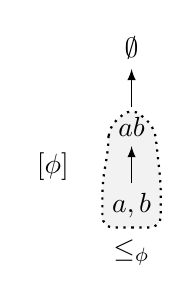
\begin{tikzpicture}
	\node at (0,-0.6){$\le_\phi$};
	\node at (0,0)(0){$a,b$};
	\node at (0,1)(1){$ab$};
	\node at (0,2)(2){$\emptyset$};
	\node at (-1, 0.5){$[\phi]$};
	\path[-latex] (0) edge (1)
	(1) edge (2);
	\fill[opacity=0.05, rounded corners=4pt]
		(0.south)--
		(0.south east)--
		(0.east)--
		(0.north east)--
		(1.east)--
		(1.north)--
		(1.west)--
		(1.south west)--
		(0.north west)--
		(0.west)--
		(0.south west)--
		(0.south);
	
	\draw[thick, dotted, rounded corners=4pt]
		(0.south)--
		(0.south east)--
		(0.east)--
		(0.north east)--
		(1.east)--
		(1.north)--
		(1.west)--
		(1.south west)--
		(0.north west)--
		(0.west)--
		(0.south west)--
		(0.south);
	\end{tikzpicture} 
	\caption{
		An agent with prior beliefs $\phi$, $[\phi]=\{a,b,ab\}$, 
		thinks outcomes $a$ and $b$ are more likely than $ab$.
		When revising by $\phi$, the result is $[\phi\re\phi]=\{a,b\}$,
		which does not fit with postulate $\ppr{\IAHB}$.
	}
	\label{fig:4-non-stability}
\end{figure}

\begin{xmpl}{Independence to already held beliefs}{4-non-iahb}
	For the set of atoms $\Atoms=\{a,b\}$,
	consider an agent whose prior beliefs are represented by the formula $\phi=a\lor b$,
	who revises according to a revision operator $\re$ that satisfies postulate $\ppr{9}$,
	and who ranks interpretations according to the total preorder $\le_\phi$ in Figure~\ref{fig:4-non-stability}.
	The agent finds out, on good authority, information consistent with $\phi$.
	On revising by $\phi$, the result is $[\phi\re\phi]=\min_{\le_\phi}[\mu] = \{a,b\}$,
	i.e., $\phi\re\phi\equiv (a\leftrightarrow\lnot b)$,
	and it is apparent that $\phi\re\phi\not\equiv\phi$ 
	and that postulate $\ppr{\IAHB}$ is not satisfied.
\end{xmpl}

In fact, postulate $\ppr{\IAHB}$ characterizes a property on interpretations
that coincides with neither of the properties introduced in this chapter,
but is familiar from Section \ref{sec:3-revision}:
recall, from there, property $\oor{5}$, saying that if two interpretations $w_1$ and $w_2$ 
are models of $\phi$, then $w_1\approx_\phi w_2$.

\begin{thm}{}{revision-representation-indifference}
	If an $\L$-revision operator $\re$ 
	satisfies postulates $\ppr{1}$ and $\ppr{3-6}$
	(i.e., is exhaustive)
	and $\as$ is a total $\L$-assignment on interpretations
	that represents it,
	then
	$\re$ satisfies postulate $\ppr{\IAHB}$ if and only if 
	$\as$ satisfies property $\oor{5}$.
\end{thm}
\begin{prf*}{}{}%
	(``$\Rightarrow$'')
	Consider an exhaustive revision operator $\re$ that satisfies postulates $\ppr{1}$ and $\ppr{3-6}$
	and, in addition, postulate $\ppr{\IAHB}$, 
	and an assignment $\as$ that represents it.
	Take two interpretations $v_1$ and $v_2$ such that $v_1,v_2\in[\phi]$. 
	Applying postulate $\ppr{\IAHB}$, it follows that $v_1,v_2\in[\phi\re\phi]$,
	and hence $v_1,v_2\in\min_{\le_\phi}[\phi]$, i.e., $v_1\approx_\phi v_2$.

	(``$\Leftarrow$'')
	Starting from an assignment $\as$ and the revision operator that represents it,
	assuming that $\oor{5}$ is satisfied, we have that $\min_{\le_\phi}[\phi] = [\phi]$,
	which implies that postulates $\ppr{\IAHB}$ is satisfied.
\end{prf*}

The ability to distinguish among models of one's prior beliefs
in terms of plausibility
points to a more graded view of what it means
to believe $\phi$. Thus, an agent might have a certain threshold of plausibility,
along the lines of what is known in epistemology
as \emph{the Lockean thesis}~\cite{Foley93},
according to which it calibrates its beliefs: 
anything above the threshold counts as part of the belief $\phi$
and anything below counts as disbelief.
This fits with the idea that an agent
might assign different degrees of plausibility to states of affairs
consistent with its belief $\phi$:
indeed, this is the point of view we endorse here,
in contrast to more standard approaches, which consider
that an agent assigns equal 
degrees of plausibility to all items of its belief.
Thus, incoming information that confirms an agent's belief might have the effect
of \emph{reinforcing} parts that are given more plausibility
at the expense of parts that are given less,
and this is the kind of situation we take to be
modeled by Example~\ref{ex:4-non-iahb}.

What would be worrying would be a revision policy
that makes an agent cycle between different viewpoints
when confronted repeatedly with the same type of information:
we will see that for revision operators satisfying $\ppr8$
this concern is unwarranted, but we must first introduce some new notation.
% If $\phi$ is a formula,
If $\phi$ is a propositional formula and $\re$ is a revision operator,
then $\phi^i$ is the formula obtained 
by revising $\phi$ by itself, using $\re$, an $i$ number of times.
Thus, $\phi^0=\phi$ and $\phi^{i+1}={\phi^i}\re{\phi}$.
Consider now the following property,
written as a postulate
meant to apply for any propositional formula $\phi$:

\begin{description}
	\item[($\ppr{\STAB}$)] There is $n\geq 1$ such that $\phi^m\equiv\phi^n$,	for every $m\geq n$.
\end{description}

Postulate $\ppr{\STAB}$, where `$\STAB$' stands for \emph{Stability},
implies that repeated revision by $\phi$ ultimately 
settles (or stabilizes) on a set of models
that does not change through subsequent revisions by $\phi$.
A revision operator $\re$ is \emph{stable} 
if it satisfies postulate $\ppr{\STAB}$. 
The following result proves relevant to the issue of stability.

\begin{prp}{}{4-inclusion-stability}
	If a revision operator $\re$ satisfies postulates $\ppr{1}$ and $\ppr{9}$,
	then $\phi^{i+1}\models\phi^i$.
\end{prp}
\begin{prf*}{}{}%
	By postulate $\ppr{1}$, we have that $\phi\re\phi\models\phi$,
	and thus $\phi^1\models\phi^0$.
	Applying postulate $\ppr{9}$,
	we have that $(\phi\re\phi)\re\phi\models(\phi\re\phi)\land\phi\models\phi\re\phi$.
	Thus, $\phi^2\models\phi^1$, and it is straightforward to see how this argument
	is iterated to get the conclusion.
\end{prf*}

If the operator $\re$ also satisfies postulate $\ppr{3}$ 
(i.e., if the revision formula
is consistent, then the revision result is also consistent),
it follows that if $\phi$ is consistent, 
then $\phi_i$ is consistent, for any $i\geq 0$.
Thus, combining this fact and Proposition \ref{prop:4-inclusion-stability},
we get that 
repeated revision by $\phi$ leads to a chain of ever more specific formulas,
i.e.,
$\emptyset\subset\dots\subseteq\mods{\phi^{i+1}}\subseteq\mods{\phi^i}\subseteq\dots\subseteq\mods{\phi^0}$.
Since a formula has a finite number of models, it falls out immediately
from this that there must be a point at which further revision by $\phi$
does not change anything.

\begin{crl}{}{stability}
	If a revision operator $\re$ satisfies postulates $\ppr{1}$ and $\ppr{8}$,
	then $\re$ is stable.
\end{crl}

Unfortunately, postulates $\ppr{11-12}$ do not guarantee stability.
Since these postulates require only that the agent places the models of $\dual{\phi}$
as the least plausible interpretations,
it becomes possible that an agent's plausibility
ranking does not hold on to a core set of interpretations
through successive revisions by $\phi$.

\begin{figure}\centering
	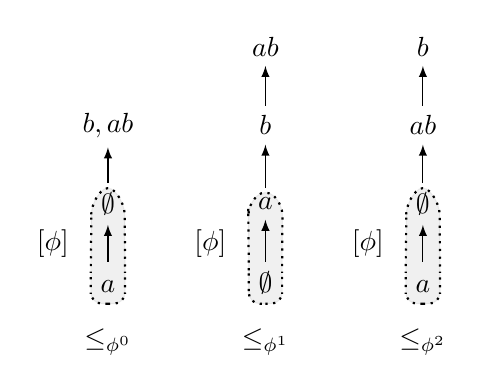
\begin{tikzpicture}
	\node at (0,-0.75){$\le_{\phi^0}$};
	\node at (0,0)(0){$a\vphantom{\emptyset}$};
	\node at (0,1)(1){$\emptyset$};
	\node at (0,2)(2){$b, ab$};
	\node at (-0.7, 0.5){$[\phi]$};
	\path[-latex] (0) edge (1)	(1) edge (2);
	\fill[draw, opacity=0.06, rounded corners=4pt]
		(0.south)--
		(0.south east)--
		(0.east)--
		(0.north east)--
		(1.east)--
		(1.north)--
		(1.west)--
		(1.south west)--
		(0.north west)--
		(0.west)--
		(0.south west)--
		(0.south);
	\draw[thick, dotted, rounded corners=4pt]
		(0.south)--
		(0.south east)--
		(0.east)--
		(0.north east)--
		(1.east)--
		(1.north)--
		(1.west)--
		(1.south west)--
		(0.north west)--
		(0.west)--
		(0.south west)--
		(0.south);
	
	\node at (2,-0.75){$\le_{\phi^1}$};
	\node at (2,0)(01){$\emptyset$};
	\node at (2,1)(11){$a$};
	\node at (2,2)(21){$b$};
	\node at (2,3)(31){$ab$};
	\node at (1.3, 0.5){$[\phi]$};
	\path[-latex] (01) edge (11)(11) edge (21)(21) edge (31);
	\fill[draw, opacity=0.06, rounded corners=4pt]
		(01.south)--
		(01.south east)--
		(01.east)--
		(01.north east)--
		(11.east)--
		(11.north)--
		(11.west)--
		(11.south west)--
		(01.north west)--
		(01.west)--
		(01.south west)--
		(01.south);
	\draw[thick, dotted, rounded corners=4pt]
		(01.south)--
		(01.south east)--
		(01.east)--
		(01.north east)--
		(11.east)--
		(11.north)--
		(11.west)--
		(11.south west)--
		(01.north west)--
		(01.west)--
		(01.south west)--
		(01.south);
	
	\node at (4,-0.75){$\le_{\phi^2}$};
	\node at (4,0)(02){$a\vphantom{\emptyset}$};
	\node at (4,1)(12){$\emptyset$};
	\node at (4,2)(22){$ab$};
	\node at (4,3)(32){$b$};
	\node at (3.3, 0.5){$[\phi]$};
	\path[-latex] (02) edge (12)(12) edge (22)(22) edge (32);
	\fill[draw, opacity=0.06, rounded corners=4pt]
		(02.south)--
		(02.south east)--
		(02.east)--
		(02.north east)--
		(12.east)--
		(12.north)--
		(12.west)--
		(12.south west)--
		(02.north west)--
		(02.west)--
		(02.south west)--
		(02.south);
	\draw[thick, dotted, rounded corners=4pt]
		(02.south)--
		(02.south east)--
		(02.east)--
		(02.north east)--
		(12.east)--
		(12.north)--
		(12.west)--
		(12.south west)--
		(02.north west)--
		(02.west)--
		(02.south west)--
		(02.south);
	\end{tikzpicture} 
	\caption{
		For an agent with prior information $\phi$, $[\phi]=\{\emptyset,a\}$,
		repeated revision by $\phi$ cycles between $\set{a}$ and $\set{\emptyset}$. 
	}
	\label{fig:postulates-89-not-stable}
\end{figure}


\begin{xmpl}{Stability}{postulates89-not-stable}
	For the set of atoms $\Atoms=\{a,b\}$
	consider an agent whose prior information is represented by the formula
	$\phi=\lnot b$,
	revises their beliefs with an operator $\re$ that satisfies postulates $\ppr{11-12}$,
	and who ranks outcomes as shown in Figure~\ref{fig:postulates-89-not-stable}.
	We have that $[\phi^0]=[\phi]=\{\emptyset,a\}$,
	$[\phi^1]=[\phi\re\phi]=\{a\}$,
	and $[\phi^2]=[\phi^1\re\phi]=\{\emptyset\}$.
	%By postulate~\R{3}, %we get that 
	By postulate $\ppr{4}$, we infer that subsequent revisions by $\phi$
	cycle between $\{a\}$ and $\{\emptyset\}$,
	i.e., 
	$[\phi^3]=\{a\}$,
	$[\phi^4]=\{\emptyset\}$,
	and so on, 
	therefore 
	thus never settling on a stable answer.
\end{xmpl}

The issue of stability suggests another dimension along which
revision operators can be analyzed, with Corollary~\ref{cor:stability}
and Example~\ref{ex:postulates89-not-stable} showing that a revision operator does not 
satisfy it trivially. 
Example~\ref{ex:postulates89-not-stable}, in particular, shows that there is 
interplay between $\le_\phi$ and $\le_{\phi'}$, if $\phi'\models\phi$,
which is relevant to the question of whether an operator is stable.
This interplay is reminiscent of topics like iterated 
revision and kinetic consistency~\cite{DarwicheP97,PeppasW16},
but pursuing it further would take us too far afield of the aims of the current work.


%%%%%%%%%%%%%%%%%%%%%%%%%%%%%%%%%%%%%%%%%%%%%%%%%%%%%%%%%%%%%%%%%%%%%%%%%%%%%%%%%%%%%%%%%%%%%%%%%%%%%%%%%%%%%%%

\section{Distance-based biased revision operators}\label{sec:4-dist-based-biased operators}
Having characterized revision operators in terms of 
assignments on interpretations, we now ask: 
what is a natural way to construct operators with such biases?
We will use the insight afforded by Theorem \ref{thm:4-biased-revision-repr}
to generate rankings on outcomes
that reflect the design principles outlined by postulates $\ppr{9-13}$.
In the process, we employ the two familiar ingredients from Section \ref{sec:2-distances}.
The first is a quasi-distance $\dd$ between interpretations,
interpreted as a measure of plausibility 
of one interpretation relative to the other.
The second ingredient is an aggregation function $\agg$,
used to compare interpretations given the distances generated by $\dd$.
Putting these two ingredients together,
we have a total $(\dd,\:\agg)$-induced $\L$-assignment $\as^{\dd,\:\agg}_\phi$,
which in turn induces the revision operator $\re^{\dd,\:\agg}$.

For quasi-distances, we will use drastic distance $\dd_\drastic$ and Hamming distance $\dd_\hamming$.
For aggregation functions, we use the ones introduced in Section \ref{sec:2-distances}, 
plus two new ones that we introduce in the following.
The \textit{$\dd$-centrality $\dd^\ctr(\phi,w)$ of $w$ with respect to $\phi$}
is defined as $\dd^\ctr(\phi, w)=\dd^\max(\phi,w)-\dd^\min(\phi, w)$.
The \emph{$\dd$-displacement $\dd^\dis(\phi,w)$ of $w$ with respect to $\phi$}
is $\dd^\dis(\phi,w)=\dd^\min(\phi,w)-\dd^\min(w^\ast,\phi)$,
where $w^\ast$ is an interpretation
such that $\dd^\min(w^\ast,\phi)$ is minimal among all
the interpretations $w'$ for which $\dd^\ctr(w',\phi)=\dd^\ctr(\phi,w)$.
Finally, 
the \textit{$\dd$-agreeability $\dd^\agr(\phi,w)$ of $w$ with respect to $\phi$} is  
defined as
$\dd^\agr(\phi,w)=\min\{\dd^\min(\phi,w),~\dd^\ctr(\phi,w)+\dd^\dis(\phi,w)\}$,
while the \textit{$\dd$-disagreeability $\dd^\dagr(\phi,w)$ of $w$ with respect to $\phi$}
is defined as 
%$\dagr(\phi,w)=\min\set{\min\dd{w,\dual{\phi}},~ 
%\ctr{w,\dual{\phi}}+\dis{w,\dual{\phi}}}$,
$\dd^\dagr(\phi,w)=m-\dd^\agr(\dual{\phi},w)$, where $m=|\Atoms|$.

\begin{xmpl}{Aggregation functions}{comparison-function}
	Take the formula $\phi=(b\rightarrow a)$, with 
	$[\phi]=\{\emptyset,a,ab\}$,
	and the interpretation $w=\emptyset$.
	The vector of Hamming distances from every model of $\phi$ to $w$ is:	
	$$
		(\dd_\hamming(\emptyset,\emptyset), \dd_\hamming(a,\emptyset),\dd_\hamming(ab,\emptyset)) = (0,1,2).
	$$
	We obtain that 
	$\dd_\hamming^\leximax(\phi,w)=(2,1,0)$
	and 
	$\dd_\hamming^\leximin(\phi,w)=(0,1,2)$.
	Additionally, we have that:
	\begin{align*}
		\dd^\min_\hamming(\phi,w)   & = 0,\\
		\dd^\max_\hamming(\phi,w)   & = 2,\\
		\dd^\ssum_\hamming(\phi, w) & = 0+1+2 = 3,\\
		\dd^\ctr_\hamming(\phi,w)   & = 2-0 = 2,\\
		\dd^\agr_\hamming(\phi, w)  & = (2-0) \cdot 0 = 0.
	\end{align*}
\end{xmpl}

Notice that the centrality of $w$ with respect to $\phi$ is $0$	
just in case $\dd^\min(\phi,w)=\dd^\max(\phi,w)$,
i.e., just in case $w$ is at equal distance to every model of $\phi$.
Thus, the agreeability index of $w$ with respect to $\phi$ is $0$
just in case $w$ is either a model of $\phi$,
or equally distanced to every model of $\phi$.

Putting these ingredients together gives us the revision operators
$\re^{\dd,\:\min}$,
$\re^{\dd,\:\leximin}$,
$\re^{\dd,\:\max}$,
$\re^{\dd,\:\leximax}$,
$\re^{\dd,\:\ssum}$,
$\re^{\dd,\:\agr}$,
$\re^{\dd,\:\dagr}$,
for $\dd\in\{\dd_\hamming,\dd_\drastic\}$.
Out of these, $\re^{\hamming,\:\min}$ is the Dalal operator
and $\re^{\drastic,\:\min}$ is the drastic operator,
presented in Section \ref{sec:3-revision}.
Thus, this perspective manages to capture 
known operators, while paving the way for some new ones.

The best way to understand these operators is to see how they rank interpretations in the universe.

\begin{table}\centering
\begin{tabular}{lccccccccc}
	%&\multicolumn{4}{c}{$[\phi]$}&&&&&\\
	\toprule
										&
	$\emptyset$ 						&
	$a$ 								& 
	$b$ 								& 
	$abc$								& 
	$\leximin$ 							& 
	$\leximax$ 							&
	$\min$								&
	$\max$								& 
	$\ssum$								\\\midrule

	$\emptyset$ 						& 
	$0$									&
	$1$									& 
	$1$									& 
	$3$									& 
	$(0,1,1,3)$							&
	$(3,1,1,0)$							&
	$0$									&	
	$3$									& 
	$5$									\\
	
	$a$									& 
	$1$									& 
	$0$									& 
	$2$									& 
	$2$									& 
	$(0,1,2,2)$							&
	$(2,2,1,0)$							&
	$0$									&
	$2$									& 
	$5$									\\

	$b$									& 
	$1$									& 
	$2$									& 
	$0$									& 
	$2$									& 
	$(0,1,2,2)$							&
	$(2,2,1,0)$							&
	$0$									&
	$2$									& 
	$5$									\\

	$c$									& 
	$1$									& 
	$2$									& 
	$2$									& 
	$2$									& 
	$(1,2,2,2)$							&
	$(2,2,2,1)$							&
	$1$									&
	$2$									& 
	$7$									\\

	$ab$								& 
	$2$									&
	$1$									& 
	$1$									& 
	$1$									& 
	$(1,1,1,2)$							&
	$(2,1,1,1)$							&
	$1$									&
	$2$									& 
	$5$									\\
	
	$ac$								& 
	$2$									&
	$1$									& 
	$3$									& 
	$1$									& 
	$(1,1,2,3)$							&
	$(3,2,1,1)$							&
	$1$									&
	$3$									&
	$7$									\\
	
	$bc$								& 
	$2$									&
	$3$									& 
	$1$									& 
	$1$									& 
	$(1,1,2,3)$							&
	$(3,2,1,1)$							&	
	$1$									&
	$3$									& 
	$7$									\\
	
	$abc$								& 
	$3$									&
	$2$									& 
	$2$									& 
	$0$									& 
	$(0,2,2,3)$							&
	$(3,2,2,0)$							&
	$0$									&
	$3$									& 
	$7$									\\\bottomrule
\end{tabular}
\caption{
	The table of Hamming distances from the models of 
	$\phi$, with $[\phi]=\{\emptyset,a,b,abc\}$,
	to every interpretation in a universe generated from three atoms.
	The aggregated values according to the aggregation functions presented in this chapter
	are also displayed.
}
\label{table:distances-example}
\end{table}


\begin{xmpl}{Distance-based biased preorders}{ops-example1}
	For the set of atoms $\Atoms=\{a,b,c\}$,
	take $\phi=(\lnot(a\land b)\land\lnot c)\lor (a\land b\land c)$,
	for which it holds that $[\phi]=\{\emptyset,a,b,abc\}$.
	For the interpretation $w=\emptyset$,
	we have that 
	$\dd^\leximin_\hamming(\phi,w)=(0,1,1,3)$,
	$\dd^\leximax_\hamming(\phi,w)=(3,1,1,0)$,
	$\dd^\min_\hamming(\phi,w)=0$,
	$\dd^\max_\hamming(\phi,w)=3$ and
	$\dd^\ssum_\hamming(\phi,w)=5$.
	The distances and aggregated distances for each
	interpretation are depicted in Table~\ref{table:distances-example}.
	Notice how the models of $\phi$
	are distributed when the interpretations are ranked according
	to the different aggregation functions used:
	we have $\emptyset\approx^{\hamming,\:\min}_\phi a$,
	since $\dd^\min_\hamming(\phi,\emptyset)=\dd^\min_\hamming(\phi,a)=0$,
	but $\emptyset<_\phi^{\hamming,\:\leximin} a$,
	since $(0,1,1,3)<_\lex(0,1,2,2)$.
	Also, we have that $c<_\phi^{\hamming,\:\max}abc$,
	$c<_\phi^{\hamming,\:\leximax}abc$
	and $ab<_\phi^{\hamming,\:\ssum}abc$, i.e.,
	models of $\phi$ are not minimal in $\le_\phi^{\hamming,\:\max}$,
	$\le_\phi^{\hamming,\:\leximax}$ and $\le_\phi^{\hamming,\:\ssum}$.
	In particular, $\le_\phi^{\hamming,\:\max}$ makes the models of $\dual{\phi}$
	(i.e., $abc$, $bc$, $ac$ and $\emptyset$)
	the least plausible interpretations. 	
\end{xmpl}

The agreement and disagreement operators 
($\re^{\dd,\:\agr}$ and $\re^{\dd,\:\dagr}$)
are simpler than they appear:
the idea behind $\re^{\dd,\:\agr}$ is to allow
interpretations other than the models of $\phi$
as the minimal elements of the preorder $\le_\phi$.
Notice that the score of an interpretation in $\le_\phi^{\dd,\:\agr}$
is $0$ if it is either a model of $\phi$,
or it is equidistant from every model of $\phi$
(i.e., its centrality is $0$) and it is the `closest'
interpretation to $\phi$ with this property. 
The disagreement operator $\re^{\dd,\:\dagr}$ works in similar fashion,
by making models of $\dual{\phi}$ and interpretations minimally equidistant to them 
the least plausible interpretations in $\le_\phi^{\dd,\:\dagr}$.

\begin{xmpl}{Agreement and disagreement operators}{ops-example2}
	If $\Atoms=\{a,b,c\}$,
	take $\phi$ such that $[\phi]=\{a,b,c\}$,
	and notice that $\emptyset$ and $abc$ 
	are both equidistant to $\phi$,
	hence their centrality is $0$.
	However, $\emptyset$ is closer to $\phi$ than $abc$
	(its displacement is $0$, compared to $abc$'s displacement of $1$),
	and $\dd_\hamming^\agr(\phi,\emptyset)=0$.
	Thus, what $\dd_\hamming^\agr$ does is to give
	a minimal score to models of $\phi$ and to the minimally equidistant
	interpretation $\emptyset$.
	By contrast, $\dd_\hamming^\dagr$ gives a maximal score
	to the models of $\dual{\phi}$ and to the maximally equidistant 
	interpretation $abc$.
\end{xmpl}

All operators proposed generate a total preorder 
$\le^{\dd,\:\agg}_\phi$ over interpretations, 
but differ in how they arrange 
models of $\phi$:
this corresponds to the different attitudes an agent can have towards
$\phi$ prior to any revision.
The operator $\re^{\hamming,\:\min}$,
known as Dalal's operator~\cite{Dalal88},
considers all models of $\phi$
as the most plausible elements in $\le_\phi^{\hamming,\:\min}$
and is the only operator of the ones considered here
for which $\phi\re\mu$ is equivalent to $\phi\land\mu$
when $\phi\land\mu$ is consistent.
%This operator is Dalal's operator~\cite{DBLP:conf/aaai/Dalal88}, and corresponds to the standard type of operator one finds in the literature.
Similarly, $\re^{\hamming,\:\leximin}$ %[{\bf SW} Check!],
also ranks models of $\phi$ as more plausible than any other interpretation,
but discriminates among models of $\phi$
% now are considered more plausible than others,
according to how typical, or representative they are 
of the general point of view expressed by $\phi$.
The operators 
$\le_\phi^{\hamming,\:\max}$
and $\le_\phi^{\hamming,\:\leximax}$
push away models of $\dual{\phi}$,
under the assumption that they are the most implausible possible worlds.
They difference between them is that $\le_\phi^{\hamming,\:\max}$ considers models of $\dual{\phi}$ equally implausible,
whereas $\le_\phi^{\hamming,\:\leximax}$ uses the more fine-grained lexicographic approach.
The operator $\re^{\hamming,\:\agr}$ 
makes models of $\phi$ the most plausible elements in $\le_\phi$ but 
does not stop here and 
also allows other interpretations on that position,
in particular certain interpretations that are equidistant to $\phi$
as per Example \ref{ex:ops-example2}.
Specifically, an interpretation can be on the lowest level of $\le_\phi$
if it either is a model of $\phi$, or is at equal distance to every model of $\phi$.
The intuition is that an interpretation equally distanced from models of $\phi$ is 
%something 
like a compromise point of view, 
with good chances of being correct if it is close to $\phi$.
The operator $\re^{\hamming,\:\dagr}$ is the dual of 
$\re^{\hamming,\:\agr}$ and,
finally, operator $\re^{\hamming,\:\ssum}$ evokes
utilitarian approaches
by choosing interpretations
that minimize the sum of the distances to each model of $\phi$,
i.e., are close to $\phi$ on an aggregate level.

Plugging in the drastic and Hamming distances  
would seem to give us a considerable number of operators,
but quick reflection shows that operators
obtained with drastic distance $\dd_\drastic$ collapse into two main categories.
%To get an idea of what these categories are,
%consider the following two types of revision operators,
%defined syntactically for a change.
To get a grasp on this fact, 
consider first the \textit{drastic revision operator $\re^\drastic$} defined,
for any propositional formulas $\phi$ and $\mu$,
as
$\phi\re^\drastic\mu=\phi\land\mu$, if $\phi\land\mu$ is consistent, and $\mu$ otherwise,
and the \textit{forgetful revision operator $\re^\forgetful$} defined as
%is defined, for $\phi\in\L_\cn$ 
%and $\mu\in\L$,
$\phi\re^\forgetful\mu=\mu$.
It is forgetful because it disregards initially held beliefs completely,
always adopting the new information $\mu$.

\begin{prp}{}{4-br-drastic-dist-ops}
	For any propositional formulas $\phi$ and $\mu$,
	it holds that 
	$\phi\re^{\drastic,\:\min}\mu
	\equiv
	\phi\re^{\drastic,\:\leximin}\mu
	\equiv
	\phi\re^{\drastic,\:\leximax}\mu
	\equiv
	\phi\re^{\drastic,\:\ssum}\mu
	\equiv
	\phi\re^\drastic\mu$.
	Moreover, $\phi\re^{\drastic,\:\agr}\mu\equiv\phi\re^\forgetful\mu$ and
	$\phi\re^{\drastic,\:\max}\mu\equiv\phi\re^{\drastic,\:\dagr}\mu\equiv
	\begin{cases}
	\phi\re^\drastic\mu,~\text{if}~\phi~\text{is complete},\\
	\phi\re^\forgetful\mu,~\text{otherwise}.
	\end{cases}
	$
\end{prp}
\begin{prf*}{}{}%
	If $\phi$ is a complete formula
	such that $[\phi]=\{v\}$,
	then 
	$\dd^\agg_\drastic(\phi,w)=\dd_\drastic(v,w)$,
	for all aggregation functions $\agg\in\{\min,\max,\leximin,\leximax,\ssum,\agr,\dagr\}$,
	and any interpretation $w$.
	In other words, it holds that:
	$$
	\dd^\agg_\drastic(\phi,w)=
		\begin{cases}
		0,~\text{if}~w=v,\\
		1,~\text{otherwise}.
		\end{cases}
	$$ 
	It is thus straightforward to conclude that if $v\in[\mu]$,
	then $[\phi\re^{\drastic,\:\max}\mu]=\{v\}=[\phi\land\mu]$,
	and if $w_0\notin[\mu]$,
	then $[\phi\re^{\drastic,\:\max}\mu]=[\mu]$.
	If $\phi$ is not complete, then we have that:
	$$
	\dd^\leximin_\drastic(\phi,w)=
		\begin{cases}
		(0,1,\dots,1),~\text{if}~w\in[\phi],\\
		(1,1,\dots,1),~\text{otherwise}.
		\end{cases}
	$$
	It is now straightforward to see that the remaining
	statements of Proposition~\ref{prop:4-br-drastic-dist-ops} hold.
\end{prf*}

We can illustrate the differential treatment of operator $\re^{\drastic,\:\max}$ 
through an example.

\begin{figure}\centering
	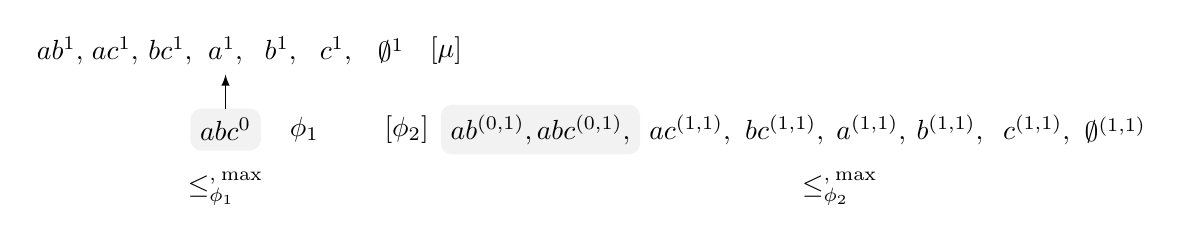
\begin{tikzpicture}			
		\node at (1, 0) {$\mods{\phi_1}$};
		\node at (2.8, 1) {$[\mu]$};
		
		\node at (0,-0.75){$\le_{\phi_1}^{\drastic,\:\max}$};
		\node at (0,0) (abc) {$abc^{{0}}$};
		\node at (-2.1, 1) (ab){$ab^{{1}},$};
		\node at (-1.4,1) (ac){$ac^{{1}},$};
		\node at (-0.7, 1) (bc){$bc^{{1}},$};
		\node at (0, 1) (a){$a^{{1}},$};
		\node at (0.7, 1) (b){$b^{{1}},$};
		\node at (1.4, 1) (c){$c^{{1}},$};
		\node at (2.1, 1) (e){$\emptyset^{{1}}$};
		
		\path[-latex] (abc) edge (a);
		\fill[opacity = 0.05, rounded corners=4]
			(abc.south) --
			(abc.south east) --
			(abc.east) --
			(abc.north east) --
			(abc.north) --
			(abc.north west) --
			(abc.west) --
			(abc.south west) --
			(abc.south);
		% \draw[thick, dotted, rounded corners=4]
		% 	(a.south)--
		% 	(b.south)--
		% 	(e.south)--
		% 	(e.south east)--
		% 	(e.east)--
		% 	(e.north east)--
		% 	(e.north)--
		% 	(e.north west)--
		% 	(c.south east)--
		% 	(c.south west)--
		% 	(b.north east)--
		% 	(b.north)--
		% 	(a.north)--
		% 	(a.north west)--
		% 	(a.west)--
		% 	(a.south west)--
		% 	(a.south);

		% \node at (-2, 0) {$\mods{\phi_2}$};
		% \node at (6.2, 0) {$[\mu]$};
%			\node at (0, 0.5){};
		
		\node at (2.3,0){$[\phi_2]$};
		\node at (7.8,-0.75){$\le_{\phi_2}^{\drastic,\:\max}$};
		\node at (4,0) (abc) {$ab^{(0,1)},abc^{(0,1)},$};
%			\node at (-2.4, 1) (ab){$ab^{{1}}$};
%			\node at (-1.6,1) (ac){$ac^{{1}}$};
		\node at (5.9, 0) (bc){$ac^{(1,1)},$};
		\node at (7.1, 0) (bc){$bc^{(1,1)},$};
		\node at (8.2, 0) (a){$a^{(1,1)},$};
		\node at (9.2, 0) (b){$b^{(1,1)},$};
		\node at (10.3, 0) (c){$c^{(1,1)},$};
		\node at (11.3, 0) (e){$\emptyset^{(1,1)}$};
		
		\fill[opacity = 0.05, rounded corners=4]
			(abc.south) --
			(abc.south east) --
			(abc.east) --
			(abc.north east) --
			(abc.north) --
			(abc.north west) --
			(abc.west) --
			(abc.south west) --
			(abc.south);
		% \draw[thick, dotted, rounded corners=4]
		% 	(a.south)--
		% 	(b.south)--
		% 	(e.south)--
		% 	(e.south east)--
		% 	(e.east)--
		% 	(e.north east)--
		% 	(e.north)--
		% 	(e.north west)--
		% 	(c.south east)--
		% 	(c.south west)--
		% 	(b.north east)--
		% 	(b.north)--
		% 	(a.north)--
		% 	(a.north west)--
		% 	(a.west)--
		% 	(a.south west)--
		% 	(a.south);
		\end{tikzpicture}                
		\caption{
			Preorders $\le^{\drastic,\:\max}_{\phi_1}$ and $\le^{\drastic,\:\max}_{\phi_2}$,
			for $\mods{\phi_1}=\set{abc}$ and $\mods{\phi_2}=\set{ab, ac, abc}$.
			Depicted as superscript to an interpretation $w$ is the vector of drastic distances $\dd_\drastic$ 
			from the models of $\phi_1$ and $\phi_2$, respectively, to $w$.
			Since $\phi_1$ is complete (i.e., has only one model), this vector consists of only one number.
			The $\max$ aggregation function uses the maximum value in the vector of distances to compare interpretations.
			}
	\label{fig:4-br-drastic-max}
\end{figure}

\begin{xmpl}{Drastic operators}{4-br-drastic-max}
	For the set of atoms $\Atoms=\{a,b,c\}$,
	consider the complete formula 
	$\phi_1 = \{a\land b\land c\}$.
	We have that:
	\begin{align*}
		\dd^\max_\drastic(\phi,w) &=\dd_\drastic(abc,w)\\
									&=\begin{cases}
										0,~\text{if}~w=abc,\\
										1,~\text{otherwise}.
									\end{cases}
	\end{align*}
	The preorder $\le_{\phi_1}^{\drastic,\:\max}$ is depicted on the left in
	Figure \ref{fig:4-br-drastic-max}.
	Consider, then, a formula
	$\phi_2 = a\land b$,
	with $[\phi_2]=\{ab, abc\}$.
	In this case we obtain, for instance, that
	$\dd^\max_\drastic(\phi,w)$, for every interpretation $w$ in the universe.
	The preorder $\le_{\phi_2}^{\drastic,\:\max}$ is depicted on the right in
	Figure~\ref{fig:4-br-drastic-max},
	which illustrates the fact that in this case $\re^{\drastic,\:\max}$ is equivalent to 
	the forgetful operator $\re^\forgetful$.
\end{xmpl}

With Hamming distance
the landscape is more diverse,
as the different attitudes the operators
assume towards models of $\phi$ lead to genuinely different
revision strategies.
Nonetheless,
certain relationships between the operators still hold, with
lexicographic operators being the most
discriminating, in the sense that they pick
formulas with fewer models, i.e., more specific formulas.
%We can get a better idea of how these operators work by looking at an example.

\begin{prp}{}{4-revision-operators-interrelations}
	If $\phi$ and $\mu$ are propositional formulas and $\dd$ is a quasi-distance,
	it holds that:
		\begin{description}
			\item[($a$)] $\phi\re^{\dd,\:\leximin}\mu\models\phi\re^{\dd,\:\min}\mu\models\phi\re^{\dd,\:\agr}\mu$,
			\item[($b$)] $\phi\re^{\dd,\:\leximax}\mu\models\phi\re^{\dd,\:\max}\mu\models\phi\re^{\dd,\:\dagr}\mu$.
		\end{description}
\end{prp}


%\begin{example}
%Take a formula $\phi$
%such that $[\phi]=\set{\emptyset,ad, abde, abcehg}$
%and a formula $\mu$ such that $[\mu]=\set{a,ab, abc,abcd,abde,abcehg}$.
%All the distances,
%together with the selection functions applied to them,
%are depicted in Table~\ref{table:table-of-distances}.
%For the preorders generated by these distances, see 
%Figures~\ref{fig:hamming-min-max}, 
%\ref{fig:hamming-leximin-leximax} 
%and \ref{fig:hamming-agre-summing}.
%
%\begin{table*}[t]\centering
%\begin{tabular}{l cccc cccccc}
%\toprule
%& 
%$\emptyset$ & 
%$ad$ & 
%$abde$ & 
%$abcehg$ & 
%$\ascending{\dd_\hamming(\phi,w)}$ &
%$\dd^\leximin_\hamming(\phi,w)$ &
%$\min$ &
%$\max$ &
%$\agr$ & 
%$\sum$\\\midrule
%$\emptyset$ & 0 & 2 & 4 & 6 &${0246}$ & ${6420}$& 0 & 6& 0& 12\\
%$ad$ & 2 & 0 & 2 & 6 &${0226}$& ${6220}$& 0 & 6 & 0& 10\\
%$abde$ & 4 & 2 & 0 & 4 &${0244}$& ${4420}$& 0 & 4 & 0 &10\\
%$abcehg$ & 6 & 6 & 4 & 0 &${0466}$& ${6640}$& 0 & 6 & 0 &16\\
%$a$ & 1 & 1 & 3 & 5 &${1135}$& ${5311}$& 1 & 5 & 4& 10\\
%$ab$ & 2 & 2 & 2 & 4 &${2224}$& ${4222}$ & 2 & 4 & 4 & 10\\
%$abc$ & 3 & 3 & 3 & 3 &${3333}$& ${3333}$& 3 & 3 & 0& 12\\
%$abcd$ & 4 & 2 & 2 & 4 &${2244}$& ${4422}$& 2 & 4 & 4& 12\\\bottomrule
%\end{tabular}
%\caption{Distances $\dd_\hamming(\phi,w)$ and the aggregation functions}
%\label{table:table-of-distances}
%\end{table*}
%%\begin{figure}\centering
%%	\begin{subfigure}[b]{0.45\textwidth}\centering
%%		\begin{tikzpicture}
%%		\node at (2.3,0)(k){$[\phi]$};
%%		\node at (1.5,2)(mu){$[\mu]$};
%%		\node at (-1.5,0) (e){$\emptyset^0$};
%%		\node at (-0.8,0) (ad){$ad^0$};
%%		\node at (0,0) (abde){$abde^0$};
%%		\node at (1.2,0) (abcehg){$abcehg^0$};
%%		\node at (0,1) (a){$a^1$};
%%		\node at (-0.5,2) (ab){$ab^2$};
%%		\node at (0,3) (abc){$abc^3$};
%%		\node at (0.5,2) (abcd){$abcd^2$};
%%		
%%		\node at (0,0.2)(1){};
%%		\node at (0,0.8)(2){};
%%		\node at (0,1.2)(3){};
%%		\node at (0,1.8)(4){};
%%		\node at (0,2.2)(5){};
%%		\node at (0,2.8)(6){};	
%%		
%%		\path
%%		(1) edge (2)
%%		(3) edge (4)
%%		(5) edge (6);
%%		
%%		\fill[fill=opacity=0.2, rounded corners=4]
%%		(e.south)--
%%		(ad.south)--
%%		(abde.south)--
%%		(abcehg.south)--
%%		(abcehg.south east)--
%%		(abcehg.east)--
%%		(abcehg.north east)--
%%		(abcehg.north)--
%%		(abde.north)--
%%		(ad.north)--
%%		(e.north)--
%%		(e.north west)--
%%		(e.west)--
%%		(e.south west)--
%%		(e.south);
%%		\fill[fill=opacity=0.5, rounded corners=4]
%%		(abcehg.south)--
%%		(abcehg.south east)--
%%		(abcehg.east)--
%%		(abcehg.north east)--
%%		(abcehg.north)--
%%		(abde.north east)--
%%		(a.south east)--
%%		(a.east)--
%%		(abcd.east)--
%%		(abc.east)--
%%		(abc.north east)--
%%		(abc.north)--
%%		(abc.north west)--
%%		(abc.west)--
%%		(ab.west)--
%%		(a.west)--
%%		(abde.west)--
%%		(abde.south west)--
%%		(abde.south)--
%%		(abcehg.south);
%%		\end{tikzpicture}   
%%		\caption{$\le_\phi^\hamming{\min}$}                 
%%	\end{subfigure}
%%	\begin{subfigure}[b]{0.45\textwidth}\centering
%%		\begin{tikzpicture}
%%		\node at (2,2.3)(k){$[\phi]$};
%%		\node at (-2,4)(k){$\mods{\dual{\phi}}$};
%%		\node at (-2,1)(mu){$[\mu]$};
%%		
%%		\node at (-1,3) (e){$\emptyset^6$};
%%		\node at (-0.2,3) (ad){$ad^6$};
%%		\node at (1,1) (abde){$abde^4$};
%%		\node at (1,3) (abcehg){$abcehg^0$};
%%		\node at (0,2) (a){$a^5$};
%%		\node at (-1,1) (ab){$ab^4$};
%%		\node at (0,0) (abc){$abc^3$};
%%		\node at (0,1) (abcd){$abcd^4$};
%%		\node at (-1.5,4)(d){$d^7$};
%%		\node at (-0.9,4)(chg){$chg^7$};
%%		\node at (0.1,4)(bcehg){$bcehg^7$};
%%		\node at (1.5,4)(abcdehg){$abcdehg^7$};
%%		
%%		\node at (0,0.2)(1){};
%%		\node at (0,0.8)(2){};
%%		\node at (0,1.2)(3){};
%%		\node at (0,1.8)(4){};
%%		\node at (0,2.2)(5){};
%%		\node at (0,2.8)(6){};	
%%		\node at (0,3.2)(7){};	
%%		\node at (0,3.8)(8){};	
%%		
%%		\path
%%		(1) edge (2)
%%		(3) edge (4)
%%		(5) edge (6)
%%		(7) edge (8);
%%		
%%		\fill[fill=opacity=0.2,rounded corners=5]
%%		(e.south)--
%%		(ad.south)--
%%		(abcehg.south)--
%%		(abde.north)--
%%		(abde.north west)--
%%		(abde.west)--
%%		(abde.south west)--
%%		(abde.south)--
%%		(abde.south east)--
%%		(abde.east)--
%%		(abde.north east)--
%%		(abcehg.south east)--
%%		(abcehg.east)--
%%		(abcehg.north east)--
%%		(abcehg.north)--
%%		(ad.north)--
%%		(e.north)--
%%		(e.north west)--
%%		(e.west)--
%%		(e.south west)--
%%		(e.south);	
%%		\fill[fill=opacity=0.5, rounded corners=5]
%%		(abcehg.north)--
%%		(abcehg.north east)--
%%		(abcehg.east)--
%%		(abcehg.south east)--
%%		(a.north east)--
%%		(a.east)--
%%		(a.south east)--
%%		(abde.north east)--
%%		(abde.east)--
%%		(abde.south east)--
%%		(abc.east)--
%%		(abc.south east)--
%%		(abc.south)--
%%		(abc.south west)--
%%		(abc.west)--
%%		(ab.south west)--
%%		(ab.west)--
%%		(ab.north west)--
%%		(a.south west)--
%%		(a.west)--
%%		(a.north west)--
%%		(abcehg.south west)--
%%		(abcehg.west)--
%%		(abcehg.north west)--
%%		(abcehg.north);
%%		
%%		\fill[fill=spanishCrimson, opacity=0.3, rounded corners=5]
%%		(d.north)--
%%		(chg.north)--
%%		(bcehg.north)--
%%		(abcdehg.north)--
%%		(abcdehg.north east)--
%%		(abcdehg.east)--
%%		(abcdehg.south east)--
%%		(abcdehg.south)--
%%		(bcehg.south)--
%%		(chg.south)--
%%		(d.south)--
%%		(d.south west)--
%%		(d.west)--
%%		(d.north west)--
%%		(d.north);
%%		\end{tikzpicture}   
%%		\caption{$\le_\phi^\hamming{\max}$}                 
%%	\end{subfigure}
%%	\caption{
%%		Preorders generated with $\min$ and $\max$
%%	}
%%	\label{fig:hamming-min-max}
%%\end{figure}
%%
%%\begin{figure}\centering
%%	\begin{subfigure}[b]{0.45\textwidth}\centering
%%		\begin{tikzpicture}
%%		\node at (1,0)(k){$[\phi]$};
%%		\node at (1,5)(mu){$[\mu]$};
%%		
%%		\node at (0,2) (e){$\emptyset^{{0246}}$};
%%		\node at (0,0) (ad){$ad^{{0226}}$};
%%		\node at (0,1) (abde){$abde^{{0244}}$};
%%		\node at (0,3) (abcehg){$abcehg^{{0466}}$};
%%		\node at (0,4) (a){$a^{{1135}}$};
%%		\node at (0,5) (ab){$ab^{{2224}}$};
%%		\node at (0,7) (abc){$abc^{{3333}}$};
%%		\node at (0,6) (abcd){$abcd^{{2244}}$};
%%		
%%		\node at (0,0.2)(1){};
%%		\node at (0,0.8)(2){};
%%		\node at (0,1.2)(3){};
%%		\node at (0,1.8)(4){};
%%		\node at (0,2.2)(5){};
%%		\node at (0,2.8)(6){};	
%%		\node at (0,3.2)(7){};
%%		\node at (0,3.8)(8){};
%%		\node at (0,4.2)(9){};
%%		\node at (0,4.8)(10){};
%%		\node at (0,5.2)(11){};
%%		\node at (0,5.8)(12){};
%%		\node at (0,6.2)(13){};
%%		\node at (0,6.8)(14){};
%%		
%%		
%%		\path
%%		(1) edge (2)
%%		(3) edge (4)
%%		(5) edge (6)
%%		(7) edge (8)
%%		(9) edge (10)
%%		(11) edge (12)
%%		(13) edge (14);
%%		
%%		\fill[fill=opacity=0.2, rounded corners=4]
%%		(ad.south)--
%%		(ad.south east)--
%%		(ad.east)--
%%		(abde.east)--
%%		(e.east)--
%%		(abcehg.east)--
%%		(abcehg.north east)--
%%		(abcehg.north)--
%%		(abcehg.north west)--
%%		(abcehg.west)--
%%		(e.west)--
%%		(abde.west)--
%%		(ad.west)--
%%		(ad.south west)--
%%		(ad.south);
%%		
%%		\fill[fill=opacity=0.5, rounded corners=4]
%%		(abde.south)--
%%		(abde.south east)--
%%		(abde.east)--
%%		(abde.north east)--
%%		(abde.north)--
%%		(e.south west)--
%%		(e.north west)--
%%		(abcehg.south)--
%%		(abcehg.south east)--
%%		(abcehg.east)--
%%		(a.east)--
%%		(ab.east)--
%%		(abcd.east)--
%%		(abc.east)--
%%		(abc.north east)--
%%		(abc.north)--
%%		(abc.north west)--
%%		(abc.west)--
%%		(abcd.west)--
%%		(ab.west)--
%%		(a.west)--
%%		(abcehg.west)--
%%		(abcehg.south west)--
%%		(e.west)--
%%		(abde.north west)--
%%		(abde.west)--
%%		(abde.south west)--
%%		(abde.south);
%%		\end{tikzpicture}   
%%		\caption{$\le_\phi^\hamming{\leximin}$}                 
%%	\end{subfigure}
%%	\begin{subfigure}[b]{0.45\textwidth}\centering
%%		\begin{tikzpicture}
%%		\node at (1,5)(k){$[\phi]$};
%%		\node at (1,1)(mu){$[\mu]$};
%%		\node at (1, 9){$\mods{\dual{\phi}}$};
%%		
%%		\node at (0,6) (e){$\emptyset^{{6420}}$};
%%		\node at (0,5) (ad){$ad^{{6220}}$};
%%		\node at (0,2) (abde){$abde^{{4420}}$};
%%		\node at (0,7) (abcehg){$abcehg^{{6640}}$};
%%		\node at (0,4) (a){$a^{{5311}}$};
%%		\node at (0,1) (ab){$ab^{{4222}}$};
%%		\node at (0,0) (abc){$abc^{{3333}}$};
%%		\node at (0,3) (abcd){$abcd^{{4422}}$};
%%		\node at (0, 8)(d1){\dots};
%%		\node at (0, 9)(d2){\dots};
%%		\node at (0, 10)(d3){\dots};
%%		
%%		\node at (0,0.2)(1){};
%%		\node at (0,0.8)(2){};
%%		\node at (0,1.2)(3){};
%%		\node at (0,1.8)(4){};
%%		\node at (0,2.2)(5){};
%%		\node at (0,2.8)(6){};	
%%		\node at (0,3.2)(7){};
%%		\node at (0,3.8)(8){};
%%		\node at (0,4.2)(9){};
%%		\node at (0,4.8)(10){};
%%		\node at (0,5.2)(11){};
%%		\node at (0,5.8)(12){};
%%		\node at (0,6.2)(13){};
%%		\node at (0,6.8)(14){};
%%		\node at (0,7.2)(15){};
%%		
%%		\path
%%		(1) edge (2)
%%		(3) edge (4)
%%		(5) edge (6)
%%		(7) edge (8)
%%		(9) edge (10)
%%		(11) edge (12)
%%		(13) edge (14)
%%		(15) edge (d1)
%%		(d1) edge (d2)
%%		(d2) edge (d3);
%%		
%%		\fill[fill=opacity=0.2,rounded corners=5]
%%		(abde.south)--
%%		(abde.south east)--
%%		(abde.east)--
%%		(abde.north east)--
%%		(abde.north)--
%%		(abcd.west)--
%%		(a.west)--
%%		(ad.south)--
%%		(ad.south east)--
%%		(ad.east)--
%%		(e.east)--
%%		(abcehg.east)--
%%		(abcehg.north east)--
%%		(abcehg.north)--
%%		(abcehg.north west)--
%%		(abcehg.west)--
%%		(e.west)--
%%		(ad.west)--
%%		(abde.west)--
%%		(abde.south west)--
%%		(abde.south);
%%		
%%		\fill[fill=opacity=0.5, rounded corners=5]
%%		(abc.south)--
%%		(abc.south east)--
%%		(abc.east)--
%%		(ab.east)--
%%		(abde.east)--
%%		(abcd.east)--
%%		(a.east)--
%%		(a.north east)--
%%		(a.north)--
%%		(ad.west)--
%%		(e.west)--
%%		(abcehg.south)--
%%		(abcehg.south east)--
%%		(abcehg.east)--
%%		(abcehg.north east)--
%%		(abcehg.north)--
%%		(abcehg.north west)--
%%		(abcehg.west)--
%%		(abcehg.south west)--
%%		(e.west)--
%%		(ad.west)--
%%		(a.west)--
%%		(abcd.west)--
%%		(abde.west)--
%%		(ab.west)--
%%		(abc.west)--
%%		(abc.south west)--
%%		(abc.south);
%%		\fill[fill=spanishCrimson, opacity=0.3, rounded corners=4]
%%		(d1.south)--
%%		(d1.south east)--
%%		(d1.east)--
%%		(d2.east)--
%%		(d3.east)--
%%		(d3.north east)--
%%		(d3.north)--
%%		(d3.north west)--
%%		(d3.west)--
%%		(d2.west)--
%%		(d1.west)--
%%		(d1.south west)--
%%		(d1.south);
%%		\end{tikzpicture}
%%		\caption{$\le_\phi^\hamming{\leximax}$}                 
%%	\end{subfigure}
%%	\caption{
%%		Preorders generated with $\leximin$ and $\leximax$
%%	}
%%	\label{fig:hamming-leximin-leximax}
%%\end{figure}
%%
%%\begin{figure}
%%	\begin{subfigure}[b]{0.45\textwidth}\centering
%%		\begin{tikzpicture}\centering
%%		\node at (-2.6,0)(k){$[\phi]$};
%%		\node at (2.4,1)(mu){$[\mu]$};
%%		
%%		\node at (-2,0) (e){$\emptyset^0$};
%%		\node at (-1.3,0) (ad){$ad^0$};
%%		\node at (-0.4,0) (abde){$abde^0$};
%%		\node at (0.8,0) (abcehg){$abcehg^0$};
%%		\node at (-1,1) (a){$a^4$};
%%		\node at (0,1) (ab){$ab^4$};
%%		\node at (2.1,0) (abc){$abc^0$};
%%		\node at (1,1) (abcd){$abcd^4$};
%%		
%%		\node at (0,0.2)(1){};
%%		\node at (0,0.8)(2){};
%%		
%%		\path
%%		(1) edge (2);
%%		
%%		\fill[fill=opacity=0.3, rounded corners=4]
%%		(e.south)--
%%		(ad.south)--
%%		(abde.south)--
%%		(abcehg.south)--
%%		(abcehg.south east)--
%%		(abcehg.east)--
%%		(abcehg.north east)--
%%		(abcehg.north)--
%%		(abde.north)--
%%		(ad.north)--
%%		(e.north)--
%%		(e.north west)--
%%		(e.west)--
%%		(e.south west)--
%%		(e.south);
%%		\fill[fill=opacity=0.3, rounded corners=4]
%%		(abcehg.south)--
%%		(abc.south)--
%%		(abc.south east)--
%%		(abc.east)--
%%		(abcd.east)--
%%		(abcd.north east)--
%%		(abcd.north)--
%%		(ab.north)--
%%		(a.north)--
%%		(a.north west)--
%%		(a.west)--
%%		(a.south west)--
%%		(abde.north west)--
%%		(abde.west)--
%%		(abde.south west)--
%%		(abde.south)
%%		(abcehg.south);
%%		\end{tikzpicture}
%%		\caption{$\le_\phi^{\hamming,\:\agr}$}
%%	\end{subfigure}
%%	\begin{subfigure}[b]{0.45\textwidth}\centering
%%		\begin{tikzpicture}
%%		\node at (-2,0)(k){$[\phi]$};
%%		\node at (2,1)(mu){$[\mu]$};
%%		\node at (-1,1) (e){$\emptyset^{12}$};
%%		\node at (-1.2,0) (ad){$ad^{10}$};
%%		\node at (0,0) (abde){$abde^{10}$};
%%		\node at (0,2) (abcehg){$abcehg^{16}$};
%%		\node at (1,0) (a){$a^{10}$};
%%		\node at (1.7,0) (ab){$ab^{10}$};
%%		\node at (-0.2,1) (abc){$abc^{12}$};
%%		\node at (1,1) (abcd){$abcd^{12}$};
%%		
%%		\node at (0,0.2)(1){};
%%		\node at (0,0.8)(2){};
%%		\node at (0,1.2)(3){};
%%		\node at (0,1.8)(4){};
%%		
%%		\path
%%		(1) edge (2)
%%		(3) edge (4);
%%		
%%		\fill[fill=opacity=0.3, rounded corners=4]
%%		(abde.south)--
%%		(ad.south)--
%%		(ad.south west)--
%%		(ad.west)--
%%		(e.west)--
%%		(e.north west)--
%%		(abcehg.south west)--
%%		(abcehg.west)--
%%		(abcehg.north west)--
%%		(abcehg.north)--
%%		(abcehg.north east)--
%%		(abcehg.east)--
%%		(abcehg.south east)--
%%		(e.north east)--
%%		(e.east)--
%%		(e.south east)--
%%		(abde.north east)--
%%		(abde.east)--
%%		(abde.south east)--
%%		(abde.south);
%%		\fill[fill=opacity=0.5, rounded corners=4]
%%		(abde.south)--
%%		(a.south)--
%%		(ab.south)--
%%		(ab.south east)--
%%		(ab.east)--
%%		(ab.north east)--
%%		(abcd.south east)--
%%		(abcd.east)--
%%		(abcd.north east)--
%%		(abcehg.south east)--
%%		(abcehg.east)--
%%		(abcehg.north east)--
%%		(abcehg.north)--
%%		(abcehg.north west)--
%%		(abcehg.west)--
%%		(abc.north west)--
%%		(abc.west)--
%%		(abc.south west)--
%%		(abde.north west)--
%%		(abde.west)--
%%		(abde.south west)--
%%		(abde.south);
%%		\end{tikzpicture}
%%		\caption{$\le_\phi^\hamming{\Sigma}$}
%%	\end{subfigure}
%%	\caption{Preorders generated with $\agr$ and $\Sigma$}
%%	\label{fig:hamming-agre-summing}
%%\end{figure}
%
%We obtain, for instance, that 
%$\ascending{\dd_\hamming{ad, \phi}}={0226}$ and
%$\ascending{\dd_\hamming{abde, \phi}}={0244}$,
%while 
%$\descending{\dd_\hamming{ad, \phi}}={6220}$ and
%$\descending{\dd_\hamming{abde, \phi}}={4420}$.
%We also have that 
%$\sum\dd_\hamming{ad, \phi}=0+2+2+6=10$ and
%$\sum\dd_\hamming{abde, \phi}=4+4+2+0=10$.
%
%Since 
%${0226}\lex{0244}$, it follows that
%$ad\le_\phi^\hamming{\leximin}abde$.
%It also holds that 
%${4420}\lex{6220}$, hence
%$abde\le_\phi^\hamming{\leximax}ad$.
%Further, it is straightforward to see that:
%\begin{align*}
%&ad\approx_\phi\hamming{\min}abde,\\
%&abde\le_\phi^\hamming{\max}ad,\\
%&ad\approx_\phi{\hamming,\:\agr}abde,\\
%&ad\approx_\phi\hamming{\ssum}abde.	
%\end{align*}
%To get $[\phi\re\mu]$,
%we take $\min_{\le_\phi}[\mu]$ with respect to each of the generated preorders
%and obtain the following results:
%\begin{table}[h]\centering
%\begin{tabular}{rll}
%	$\mods{\re^{\hamming,\:\min}{\phi}{\mu}}=$&
%	$\min_{\le_\phi^\hamming{\min}}[\mu]$&=
%	$\set{abde, abcehg}$,\\
%	$\mods{\re^{\hamming,\:\leximin}{\phi}{\mu}}=$&
%	$\min_{\le_\phi^\hamming{\leximin}}[\mu]$&=
%	$\set{abde}$,\\
%	$\mods{\re^{\hamming,\:\max}{\phi}{\mu}}=$&
%	$\min_{\le_\phi^\hamming{\max}}[\mu]$&=
%	$\set{abc}$,\\
%	$\mods{\re^{\hamming,\:\leximax}{\phi}{\mu}}=$&
%	$\min_{\le_\phi^\hamming{\leximax}}[\mu]$&=
%	$\set{abc}$,\\
%	$\mods{\re{\hamming,\:\agr}{\phi}{\mu}}=$&
%	$\min_{\le_\phi^{\hamming,\:\agr}}[\mu]$&=
%	$\set{abde, abcehg, abc}$,\\
%	$\mods{\re^{\hamming,\:\Sigma}{\phi}{\mu}}=$&
%	$\min_{\le_\phi^\hamming{\Sigma}}[\mu]$&=
%	$\set{a, ab, ad, abde}$.
%\end{tabular}
%\end{table}
%\end{example}

%\noindent 
%The relationship between the different operators is
%depicted in Figure~\ref{fig:relationship-operators}.
%Lexicographic operators are the most
%discriminating, in the sense that they pick
%formulas with fewer models (i.e., more specific formulas).

%% \begin{figure}\centering
%% \begin{tikzpicture}
%% \node at (0,0)(lmin){$\re{\dd}{\leximin}$};
%% \node at (1.5,0)(min){$\re{\dd}{\min}$};
%% \node at (3,0)(agr){$\re{\dd}{\agr}$};
%% \node at (4.3,0)(lmax){$\re{\dd}{\leximax}$};
%% \node at (5.8,0)(max){$\re{\dd}{\max}$};
%% \node at (7,0)(sum){$\re{\dd}{\ssum}$};
%% \path[->]	(lmin) edge (min)	(min) edge (agr)	(lmax) edge (max);
%% \end{tikzpicture}
%% \caption{
%% An arrow from $x$ to $y$ indicates that the output
%% of operator $x$ implies output of operator $y$ 
%% for the same input
%% }
%% \label{fig:relationship-operators}
%% \end{figure}

All operators generate total preorders over interpretations,
so by Theorem \ref{thm:3-revision-repr-km-total}
they all satisfy postulates $\ppr{1}$ and $\ppr{3-6}$.
Satisfaction with respect to the newly introduced postulates 
is clarified below, but before we state the result 
we introduce a property of distances that will be useful 
in settling the matter with respect to neutrality.
This property is expected to hold for any interpretations $w_1$ and $w_2$
and renaming $\rnm$ of the atoms in $\Atoms$:

\begin{description}
	\item[($\ood{\NEUT}$)] $\dd(w_1,w_2)=\dd(\rnm(w_1), \rnm(w_2))$.
\end{description}

A quasi-distance $\dd$ is \textit{neutral} if it satisfies property $\ood{\NEUT}$.
With this in hand, we can introduce the result.

\begin{table}\centering
	\begin{tabular}{rcccccccc}\toprule
		&
		$\ppr{9}$					&
		$\ppr{10}$					&
		$\ppr{11}$					&
		$\ppr{12}$					&
		$\ppr{13}$					&
		$\ppr{\NEUT}$					&
		$\ppr{\IAHB}$					&
		$\ppr{\STAB}					$
									\\\midrule
		
		$\re^{\hamming,\:\min}$ 	& 
		$\checkmark$				&
		$\checkmark$				&
		$\times$					&
		$\times$					&
		$\checkmark$				&
		$\checkmark$				&
		$\checkmark$				&
		$\checkmark$				\\
		
		$\re^{\hamming,\:\leximin}$	&
		$\checkmark$				&
		$\times$					&
		$\times$					&
		$\times$					&
		$\checkmark$				&
		$\checkmark$				&
		$\times$					&
		$\checkmark$				\\
		
		$\re^{\hamming,\:\agr}$		&
		$\times$					&
		$\checkmark$				&
		$\times$					&
		$\times$					&
		$\checkmark$				&
		$\checkmark$				&
		$\checkmark$				&	
		$\checkmark$				\\
		
		$\re^{\hamming,\:\max}$	&
		$\times$					&
		$\times$					&
		$\checkmark$				&
		$\checkmark$				&
		$\times$					&
		$\checkmark$				&
		$\times$					&
		$\checkmark$				\\
		
		$\re^{\hamming,\:\leximax}$	&
		$\times$					&
		$\times$					&
		$\times$					&
		$\checkmark$				&
		$\times$					&
		$\checkmark$				&
		$\times$					&
		$\checkmark$				\\
		
		$\re^{\hamming,\:\dagr}$	&
		$\times$					&
		$\times$					&
		$\checkmark$				&
		$\times$					&
		$\times$					&
		$\checkmark$				&
		$\checkmark$				&
		$\checkmark$				\\
		
		$\re^{\hamming,\:\ssum}$	&
		$\times$					&
		$\times$					&
		$\times$					&
		$\times$					&
		$\checkmark$				&
		$\checkmark$				&
		$\times$					&
		$\checkmark$				\\
		
		$\re^\drastic$				&
		$\checkmark$				&
		$\checkmark$				&
		$\times$					&
		$\times$					&
		$\checkmark$				&
		$\checkmark$				&
		$\checkmark$				&
		$\checkmark$				\\
		
		$\re^\forgetful$			&
		$\times$					&
		$\checkmark$				&
		$\checkmark$				&
		$\times$					&
		$\checkmark$				&
		$\checkmark$				&
		$\checkmark$				&
		$\checkmark$				\\\bottomrule
	\end{tabular}
\caption{
	Satisfaction of postulates for the biased operators $\re^{\dd,\:\agg}$
	described in this chapter.
	We include rows for operators $\re^\drastic$ and $\re^\forgetful$ rather than 
	have separate rows for the operators generated using drastic distance $\dd_\drastic$,
	with the understanding given by Proposition \ref{prop:4-br-drastic-dist-ops}
	that they collapse, in one way or another, into one of these two.
	}
\label{tab:4-br-biased-ops-postulates}
\end{table}

\begin{prp}{}{4-br-biased-distance-ops-postulates}
	For $\dd\in\{\dd_\drastic,\dd_\hamming\}$ 
	and $\agg\in\{\min, \leximin, \max, \leximax,\agr, \dagr, \ssum\}$,
	the operators $\re^{\dd,\:\agg}$ satisfy
	postulates $\ppr{9-13}$, $\ppr{\NEUT}$, $\ppr{\IAHB}$ and $\ppr{\STAB}$ 
	as shown in Table \ref{tab:4-br-biased-ops-postulates}.
\end{prp}
\begin{prf*}{}{}%
	We will use Theorem \ref{thm:4-biased-revision-repr} to show that the operators
	arrange interpretations in the patters described by the properties $\oor{7-11}$.

	It is already known that $\le_\phi^{\hamming,\:\min}$, known as Dalal's operator \cite{Dalal88},
	satisfies postulate $\ppr{6}$, which implies that it satisfies postulates $\ppr{9}$ and $\ppr{10}$. 
	To see why the operator $\re^{\hamming,\:\leximin}$ satisfies $\ppr{9}$,
	notice that if $w_1\in[\phi]$ and $w_2\notin[\phi]$, 
	then the first element in $\dd^\leximin_\hamming(\phi,w_1)$ is $0$,
	while the first element in $\dd^\leximin_\hamming(\phi,w_2)$ is 
	strictly greater than $0$.
	This implies that 
	$\dd^\leximin_\hamming(\phi,w_1)<_\lex\dd^\leximin_\hamming(\phi,w_2)$,
	which in turn implies that $w_1<_\phi^{\hamming,\:\leximin}w_2$.   
	Hence property $\oor{7}$ is satisfied,
	which implies that postulate $\ppr{9}$ is satisfied.	
	For $\re^{\hamming,\:\leximin}$ and postulate $\ppr{10}$, take
	$[\phi]=\{a,b,ab\}$ and $[\mu]=\{a,b,ab\}$.
	We get that $[\phi \re^{\hamming,\:\leximin}\mu]=\{a,b\}$
	and thus 
	$\phi\land\mu\not\models\phi \re^{\hamming,\:\leximin}\mu$.
	The operator $\re^{\hamming,\:\agr}$ satisfies postulate $\ppr{10}$ because
	it makes all models of $\phi$, and potentially other interpretations as well
	(which is the reason why it does not satisfy postulate $\ppr{9}$),
	as the equally most plausible interpretations in $\le_\phi^{\hamming,\:\agr}$. 
	Since all these operators place the models of $\phi$ on the lowest levels of 
	$\le_\phi$, they all satisfy postulate $\ppr{13}$.
	
	To see why postulates $\ppr{11}$ and $\ppr{12}$ are not satisfied by
	$\re^{\hamming,\:\agg}$,
	for $\agg\in\{\min,\leximin,\agr\}$,
	it is sufficient to 
	notice that these operators do not make models of $\dual{\phi}$ as the least plausible interpretations
	in $\le_\phi^{\hamming,\:\agg}$. Thus, if $\phi=a\lor b$, then $\dual{\phi}$ shares some models
	with $\phi$, yet these models (along with all other models of $a\lor b$)
	will be among the most plausible interpretations
	in $\le_\phi^{\hamming,\:\min}$, $\le_\phi^{\hamming,\:\leximin}$ and $\le_\phi^{\hamming,\:\agr}$,
	due to how these preorders are defined.
	The one exception is the forgetful operator $\re^\forgetful$, 
	which satisfies $\ppr{11}$ trivially.
	
	The case for $\re^{\hamming,\:\max}$, $\re^{\hamming,\:\leximax}$
	and $\re^{\hamming,\:\dagr}$ is analogous to the one for 
	$\re^{\hamming,\:\min}$, $\re^{\hamming,\:\leximin}$
	and $\re^{\hamming,\:\agr}$, as they can be seen as duals of each other.
	For the operator $\re^{\hamming,\:\ssum}$ and postulates $\ppr{9-10}$, 
	take $[\phi]=\{a,b,c\}$ and $[\mu]=\{\emptyset,a,b,c\}$. 
	We get that $[\phi\re^{\hamming,\:\ssum}\mu]=\{\emptyset\}$,
	as $\emptyset$ minimizes the sum of the Hamming distances to the models 
	of $\phi$.
	For postulates $\ppr{11-12}$, take $[\mu']=\{\emptyset,ab,ac,bc\}$.
	For $\re^{\hamming,\:\ssum}$ and $\ppr{13}$,
	notice that adding $v$ to $[\phi]$ creates a new column for $v$
	in the table of distances, in which the distance corresponding to $v$
	is $0$, i.e., the score assigned to $w'$ in $\le_{\phi\lor\phi'}^{\hamming,\:\ssum}$ 
	does not increase with respect to $\le_\phi^\hamming{\ssum}$. 
	Satisfaction of $\ppr{\IAHB}$ and $\ppr{\STAB}$ is straightforward, keeping in mind
	how the various operators arrange the models of $\phi$ in the generated preorders.

	For the neutrality postulate $\ppr{\NEUT}$,
	it is straightforward to see that the drastic and Hamming distances
	are neutral.
	Furthermore, if $\dd$ is neutral,
	then it follows straightforwardly that 
	$\dd^{\agg}(\phi,w)=\dd^{\rnm}(\rnm(\phi),\rnm(w))$,
	for any $w\in\U$,
	and 
	%it is straightforward to see that 
	$w_1\le_\phi^{\dd,\:\agg}w_2$ iff $\rnm(w_1)\le^{\dd,\:\agg}_{\rnm(\phi)}\rnm(w_2)$,
	for all aggregation functions introduced so far.
	Thus, the preorders $\le_\phi^{\dd,\:\agg}$ satisfy property $\oor{\NEUT}$
	and, by Theorem \ref{thm:4-biased-revision-repr},
	the operators represented by them satisfy postulate $\ppr{\NEUT}$.
\end{prf*}

It should be kept in mind that neutrality is not
guaranteed by the standard postulates $\ppr{1-6}$,
or by any of the other postulates introduced so far,
but the way in which concrete operators are usually defined
(i.e., by appeal to neutral distances) indicates that neutrality is
part of our basic understanding of how a revision operator
should behave.
And, in general, there seems to be no a priori reason for
looking at non-neutral operators.
However, we will see in Chapter \ref{ch:6} 
that such operators cannot be avoided
when we move to a fragment of propositional logic.

% Neutrality of $\dd$ is sufficient to guarantee that the assignment 
% generated using it is also neutral.
% \begin{prp}{}{neutrality-of-distance-implies-neutrality-of-order}
% 	If $\dd$ is a quasi-distance
% 	and $\agg$ is an aggregation function such that 
% 	$\agg\in\{\min, \max, \leximin, \leximax, \agr, \ssum\}$,
% 	the preorder $\le_\phi^{\dd,\:\agg}$ is neutral. 	
% \end{prp}
% \begin{prf*}{}{}%
% 	Notice that if $\dd$ is neutral,
% 	then $\dd(\phi,w)=\dd(\rnm(w),\rnm(\phi))$,
% 	for any interpretation $w$,
% 	and it is straightforward to see that 
% 	$w_1\le_\phi^{\dd,\:\agg}w_2$ iff $\rnm(w_1)\le^{\dd,f}_{\rnm(\phi)}\rnm(w_2)$,
% 	for all of the aggregation functions mentioned.
% \end{prf*}










\section{Related work}\label{sec:4-rw}
The idea that revision postulate $\ppr{2}$ sometimes leads to counterintuitive results 
has been remarked upon before.

\begin{xmpl}{John}{4-john}
	Consider the example of John, proposed by Ferm\'e and Hansson:

	\begin{quote}
		John is a neighbour about whom I initially know next to nothing.

		\emph{Case 1}: I am told that he goes home from work by taxi every day ($t$). 
		This makes me believe that he is a rich man ($r$).

		\emph{Case 2}: When told $t$, I am also told that John is a driver by profession ($d$). 
		In this case I am not made to believe that he is a rich man ($r$).
		\cite[p.~45]{FermeH18}
	\end{quote}
	
	In our terminology, the set of atoms is $\Atoms=\{t,r,d\}$.
	The agent's initial beliefs are $\phi$: we are not told what $\phi$ is,
	but we are led to believe that it is consistent with $t$, $r$ and $d$.
	Let us assume that $\phi=\top$.
	There are two instances of revision, once by $\mu_1 = t$,
	and then by $\mu_2 = t\land d$.
	We are told that $\phi\re\mu_1\models r$, but $\phi\re\mu_2\not\models r$.
	Assuming the agent is revising according to a total preorder $\le_{\phi}$ on interpretations,
	the claims above translate to 
	$\min_{\le_{\phi}}\{t,tr,td,trd\} \subseteq\{r,tr,rd,trd\}$,
	but $\min_{\le_{\phi}}\{td,trd\} \nsubseteq\{r,tr,rd,trd\}$.
	This is not possible if the agent considers all interpretations as equally plausible:
	the agent must consider, for instance, 
	that $tr<_{\phi}td$ and $tr<_{\phi}tdr$.
	This is clearly in conflict with postulate $\ppr{2}$.
\end{xmpl}

Ferm\'e and Hansson explain Example \ref{ex:4-john}
by appeal to a type of cognitive attitude that an agent might 
plausibly adopt when revising:

\begin{quote}
	When we acquire a new belief that does not contradict our previous beliefs 
	(such as $t$ in the example), we often include in the outcome 
	some additional belief (such as $r$ in the example) 
	that does not follow deductively but nevertheless serves to make the belief
	set more complete and/or more coherent. \cite[p.~45]{FermeH18}
\end{quote}

Presumably, John jumps to conclusions according to some stereotypical 
images about rich people and cars.
This is exactly the type of attitude exhibited in Examples \ref{ex:4-asthma-symptoms}
and \ref{ex:4-heuristic-availability}. Later in the same section, 
Ferm\'e and Hansson also present another example.

\begin{xmpl}{Valentina}{4-valentina}
	Consider the example of Valentina, proposed by Ferm\'e and Hansson:

	\begin{quote}
		Valentina was uncertain whether or not her husband is unfaithful to
		her ($u$), but she still believed that her husband loves her ($l$). 
		However, when she learnt that he is unfaithful to her, 
		she lost her belief that he loves her.
		\cite[p.~45]{FermeH18}
	\end{quote}
	
	In our terminology, 
	the set of atoms is $\Atoms=\{u,l\}$,
	Valentina's prior belief is $\phi=l$, 
	the new information is $\mu=u$, and 
	Valentina's posterior information after revision is
	$\phi\re\mu \equiv u\land\lnot l$,
	whereas postulate $\ppr{2}$ requires that $\phi\re\mu\equiv u\land l$.
\end{xmpl}

Right after presenting this example
Ferm\'e and Hansson mention that postulate $\ppr{2}$, 
or, as they call it, the \emph{expansion property of revision},
``has been much less discussed than the recovery property of contraction, 
but it is no less problematic and no less difficult to remove from the AGM framework'' 
\cite[p.~45]{FermeH18}.

A response to these kinds of examples has been the framework of \emph{abductive expansion}
\cite{Pagnucco94}, in which addition of a new item of knowledge must come with a 
justification, or explanation for the new belief.
A semantic model for this operation is sketched in terms of Groves' system of spheres \cite{Grove88},
but not much more detail is added.
Other than this, there are few other works considering revision operators 
that do not satisfy the classical postulate $\ppr{2}$ \cite{Ryan96,BenferhatLP05}.
As shown above, the acknowledgement that 
deviations from $\ppr{2}$ make sense is not entirely foreign,
but the idea such deviations correspond to possible 
epistemic attitudes and can be realized through distance-based
approaches has, to the best of our knowledge, 
not been considered in any systematic detail before.


















\section{Conclusion}
In this chapter we have looked at the classical  revision postulates
from the point of view of what they assume about an agent's 
attitude towards its initial beliefs,
and argued that this attitude is embedded in a specific postulate,
i.e., the standard postulate $\ppr{2}$.
By varying this postulate
and calling attention to a commonly overlooked neutrality property,
we were able to put forward and 
characterize a wide range of revision operators,
and refine previously entangled intuitions in the process.
We also showed that this level of analysis is needed when working
in restricted fragments of propositional logic,
where postulate $\ppr{2}$ cannot be satisfied and must therefore
be broken down into two separate components (postulates $\ppr{7-8}$ in the current work).
The aggregation functions used to construct revision operators
recall methods to rank outcomes in decision theory. 
Analysis of the new operators also 
uncovered the principles of indifference to already held beliefs ($\ppr{\IAHB}$) and
stability ($\ppr{\STAB}$). Further work is needed to link these notions to the other 
postulates, to map out their interplay 
and to provide them with semantic characterizations.
Following the line of reasoning initiated in the previous section,
a natural follow-up would be to consider the proposed
postulates in fragments of propositional logic 
and to look for characterizations in terms of 
preorders on outcomes.

Discussions of stability and biases notwithstanding,
one might still question the rationale behind doubting 
postulate $\ppr{2}$:
indeed, why fix something if it is not broken?
In response, we will see in Chapter \ref{ch:6} that 
there situations where revision is warranted, but in which
postulates $\ppr{9-10}$ \emph{cannot} occur together.
In Chapter \ref{ch:6} we will look at revision of Horn formulas:
as mentioned in the introduction,
there is good reason to want to do 
revision on such specialized formulas,
and we will see that postulate $\ppr{2}$ is at odds 
with the expressibility requirements of 
such a revision operator.
